% \newcommand{\compacttitlespacing}{0} %disable when we need room for authors
\documentclass[sigconf]{acmart}
\settopmatter{printacmref=false}
% defining the \BibTeX command - from Oren Patashnik's original BibTeX documentation.
\def\BibTeX{{\rm B\kern-.05em{\sc i\kern-.025em b}\kern-.08emT\kern-.1667em\lower.7ex\hbox{E}\kern-.125emX}}
\usepackage{multirow}
\usepackage[normalem]{ulem}
\useunder{\uline}{\ul}{}
\usepackage{nicefrac}
\usepackage{siunitx}
\usepackage{array,framed}
\usepackage{booktabs}
\usepackage{
  color,
  float,
  epsfig,
  wrapfig,
  graphics,
  graphicx,
  subcaption
}
% \usepackage[dvipsnames]{xcolor}
\usepackage{textcomp,amssymb}
\usepackage{setspace}
% \usepackage{amsfonts}
\usepackage{latexsym,fancyhdr,url}
\usepackage{enumerate}
\usepackage{algorithm2e}
\usepackage{algpseudocode}
\usepackage{graphics}
\usepackage{xparse} % argument parsing -- \edist
\usepackage{xspace}
\usepackage{multirow}
\usepackage{csvsimple}
\usepackage{balance}
% \usepackage{flushend}
% \usepackage{mathptmx,avant}

%%%% Tikz variables, pgfplot
\usepackage{
  tikz,
  pgfplots,
  pgfplotstable
}
\usepackage{hyperref}

\usetikzlibrary{
  shapes.geometric,
  arrows,
  external,
  pgfplots.groupplots,
  matrix
}

\pgfplotsset{compat=1.9}
% \tikzexternalize[prefix=images/]
% \tikzexternalenable

%\pagenumbering{arabic}
% \pagestyle{plain}

\usepackage{mathtools,}
\DeclarePairedDelimiter\abs{\lvert}{\rvert}
\DeclarePairedDelimiter\norm{\lVert}{\rVert}

% \setmathfont{Latin Modern Math}[version=lm]
\DeclareMathAlphabet{\mathcal}{OMS}{cmsy}{m}{n}
% \DeclareSymbolFont{operators}{T1}{cmr}{m}{n}
% \DeclareSymbolFont{letters}{OML}{cmm}{m}{it}
% \DeclareSymbolFont{symbols}{OMS}{cmsy}{m}{n}
% \DeclareSymbolFont{largesymbols}{OMX}{cmex}{m}{n}

% \usepackage{times}

% \setmathcal{Arial}

% TO deal with the weird flow of boxes
% \brokenpenalty=1000
% \clubpenalty=1000
% \widowpenalty=10
\DeclareGraphicsExtensions{%
    .png,.PNG,%
    .pdf,.PDF,%
    .jpg,.mps,.jpeg,.jbig2,.jb2,.JPG,.JPEG,.JBIG2,.JB2}

\usepackage{xparse}
\newcommand{\bnm}{\begin{newmath}}
\newcommand{\enm}{\end{newmath}}

\newcommand{\bea}{\begin{eqnarray*}}%
\newcommand{\eea}{\end{eqnarray*}}%

\newcommand{\bne}{\begin{newequation}}
\newcommand{\ene}{\end{newequation}}

\newcommand{\bal}{\begin{newalign}}
\newcommand{\eal}{\end{newalign}}

\newenvironment{newalign}{\begin{align}%
\setlength{\abovedisplayskip}{4pt}%
\setlength{\belowdisplayskip}{4pt}%
\setlength{\abovedisplayshortskip}{6pt}%
\setlength{\belowdisplayshortskip}{6pt} }{\end{align}}

\newenvironment{newmath}{\begin{displaymath}%
\setlength{\abovedisplayskip}{4pt}%
\setlength{\belowdisplayskip}{4pt}%
\setlength{\abovedisplayshortskip}{6pt}%
\setlength{\belowdisplayshortskip}{6pt} }{\end{displaymath}}

\newenvironment{neweqnarrays}{\begin{eqnarray*}%
\setlength{\abovedisplayskip}{-4pt}%
\setlength{\belowdisplayskip}{-4pt}%
\setlength{\abovedisplayshortskip}{-4pt}%
\setlength{\belowdisplayshortskip}{-4pt}%
\setlength{\jot}{-0.4in} }{\end{eqnarray*}}

\newenvironment{newequation}{\begin{equation}%
\setlength{\abovedisplayskip}{4pt}%
\setlength{\belowdisplayskip}{4pt}%
\setlength{\abovedisplayshortskip}{6pt}%
\setlength{\belowdisplayshortskip}{6pt} }{\end{equation}}


\newcounter{ctr}
\newcounter{savectr}
\newcounter{ectr}

\newenvironment{newitemize}{%
\begin{list}{\mbox{}\hspace{5pt}$\bullet$\hfill}{\labelwidth=15pt%
\labelsep=4pt \leftmargin=12pt \topsep=3pt%
\setlength{\listparindent}{\saveparindent}%
\setlength{\parsep}{\saveparskip}%
\setlength{\itemsep}{3pt} }}{\end{list}}


\newenvironment{newenum}{%
\begin{list}{{\rm (\arabic{ctr})}\hfill}{\usecounter{ctr} \labelwidth=17pt%
\labelsep=5pt \leftmargin=22pt \topsep=3pt%
\setlength{\listparindent}{\saveparindent}%
\setlength{\parsep}{\saveparskip}%
\setlength{\itemsep}{2pt} }}{\end{list}}

%%%%%%%%%%%%%%%%%%%%%%%%%%%%%%%%%%%%%%%%%%%%%%%%%%%%%%%%%%%%%%%%%%%%%%%%%%%%%%
%
% Figure and table macros
%

\newcounter{mytable}
\def\mytable{\begin{centering}\refstepcounter{mytable}}
\def\endmytable{\end{centering}}

\def\mytablecaption#1{\vspace{2mm}
  \centerline{Table \arabic{mytable}.~{#1}}
  \vspace{6mm}
  \addcontentsline{lot}{table}{\protect\numberline{\arabic{mytable}}~{#1}}
}


\newcounter{myfig}
\def\myfig{\begin{centering}\refstepcounter{myfig}}
\def\endmyfig{\end{centering}}

\def\myfigcaption#1{
             \vspace{2mm}
             \centerline{\textsf{Figure \arabic{myfig}.~{#1}}}
             \vspace{6mm}
             \addcontentsline{lof}{figure}{\protect\numberline{\arabic{myfig}}~{#1}}}


\newlength{\saveparindent}
\setlength{\saveparindent}{\parindent}
\newlength{\saveparskip}
\setlength{\saveparskip}{\parskip}

\newcommand{\decOracle}{\textbf{Dec}}

\newcommand{\negsmidge}{{\hspace{-0.1ex}}}
\newcommand{\cdotsm}{\negsmidge\negsmidge\negsmidge\cdot\negsmidge\negsmidge\negsmidge}

\def\suchthatt{\: :\:}
\newcommand{\E}{{\rm I\kern-.3em E}}
\newcommand{\Prob}[1]{{\Pr\left[\,{#1}\,\right]}}
\newcommand{\Probb}[2]{{\Pr}_{#1}\left[\,{#2}\,\right]}
\newcommand{\CondProb}[2]{{\Pr}\left[\: #1\:\left|\right.\:#2\:\right]}
\newcommand{\CondProbb}[2]{\Pr[#1|#2]}
\newcommand{\ProbExp}[2]{{\Pr}\left[\: #1\:\suchthatt\:#2\:\right]}
\newcommand{\Ex}[1]{{\textnormal{E}\left[\,{#1}\,\right]}}
\newcommand{\Exx}{{\textnormal{E}}}
\newcommand{\given}{\ensuremath{\,\big|\,}}


\newcommand{\true}{\mathsf{true}}
\newcommand{\false}{\mathsf{false}}
\def\negl{\mathsf{negl}}


\newcommand{\secref}[1]{\mbox{Section~\ref{#1}}}
\newcommand{\appref}[1]{\mbox{Appendix~\ref{#1}}}
\newcommand{\thref}[1]{\mbox{Theorem~\ref{#1}}}
\newcommand{\defref}[1]{\mbox{Definition~\ref{#1}}}
\newcommand{\corref}[1]{\mbox{Corollary~\ref{#1}}}
\newcommand{\lemref}[1]{\mbox{Lemma~\ref{#1}}}
\newcommand{\clref}[1]{\mbox{Claim~\ref{#1}}}
\newcommand{\propref}[1]{\mbox{Proposition~\ref{#1}}}
\newcommand{\factref}[1]{\mbox{Fact~\ref{#1}}}
\newcommand{\remref}[1]{\mbox{Remark~\ref{#1}}}
\newcommand{\figref}[1]{\mbox{Figure~\ref{#1}}}
\renewcommand{\algref}[1]{\mbox{Algorithm~\ref{#1}}}
% \newcommand{\eqref}[1]{\mbox{Equation~(\ref{#1})}}
% Have to use \renewcommand because exists already in amsmath
\renewcommand{\eqref}[1]{\mbox{Equation~(\ref{#1})}}
\newcommand{\consref}[1]{\mbox{Construction~\ref{#1}}}
\newcommand{\tabref}[1]{\mbox{Table~\ref{#1}}}

\newcommand{\get}{{\:{\leftarrow}\:}}
\newcommand{\gett}[1]{\:{\leftarrow}_{#1}\:}
\newcommand{\getsr}{{\:{\leftarrow{\hspace*{-3pt}\raisebox{.75pt}{$\scriptscriptstyle\$$}}}\:}}
\newcommand{\getm}{{\:\leftarrow_{\mdist}\:}}
\newcommand{\getd}{{\:\leftarrow_{\ddist}\:}}
%\newcommand{\getm}{{\:{\leftarrow{\hspace*{-3pt}\raisebox{.75pt}{$\scriptscriptstyle \mdist$}}}\:}}
\newcommand{\getk}{{\:\leftarrow_{\kdist}\:}}
%\newcommand{\getk}{{\:{\leftarrow{\hspace*{-3pt}\raisebox{.75pt}{$\scriptscriptstyle \kdist$}}}\:}}
\newcommand{\getp}{{\:\leftarrow_{p}\:}}



\newcommand{\gamesfontsize}{\small}
\newcommand{\fpage}[2]{\framebox{\begin{minipage}[t]{#1\textwidth}\setstretch{1.1}\gamesfontsize  #2 \end{minipage}}}
\newcommand{\mpage}[2]{\begin{minipage}[t]{#1\textwidth}\setstretch{1.1}\gamesfontsize  #2 \end{minipage}}

\newcommand{\hpages}[3]{\begin{tabular}{cc}\begin{minipage}[t]{#1\textwidth} #2 \end{minipage} & \begin{minipage}[t]{#1\textwidth} #3 \end{minipage}\end{tabular}}

\newcommand{\hpagess}[4]{
        \begin{tabular}[t]{c@{\hspace*{.5em}}c}
        \begin{minipage}[t]{#1\textwidth}\gamesfontsize #3 \end{minipage}
        &
        \begin{minipage}[t]{#2\textwidth}\gamesfontsize #4 \end{minipage}
        \end{tabular}
    }

\newcommand{\hpagesss}[6]{
        \begin{tabular}[t]{c@{\hspace*{.5em}}c@{\hspace*{.5em}}c@{\hspace*{.5em}}c}
        \begin{minipage}[t]{#1\textwidth}\gamesfontsize #4 \end{minipage}
        &
        \begin{minipage}[t]{#2\textwidth}\gamesfontsize #5 \end{minipage}
        &
        \begin{minipage}[t]{#3\textwidth}\gamesfontsize #6 \end{minipage}
        \end{tabular}
    }

\newcommand{\hpagessss}[8]{
        \begin{tabular}{c@{\hspace*{.5em}}c@{\hspace*{.5em}}c@{\hspace*{.5em}}c}
        \begin{minipage}[t]{#1\textwidth}\gamesfontsize #5 \end{minipage}
        &
        \begin{minipage}[t]{#2\textwidth}\gamesfontsize #6 \end{minipage}
        &
        \begin{minipage}[t]{#3\textwidth}\gamesfontsize #7 \end{minipage}
        &
        \begin{minipage}[t]{#4\textwidth}\gamesfontsize #8 \end{minipage}
        \end{tabular}
    }


\newcommand{\hfpages}[3]{\hfpagess{#1}{#1}{#2}{#3}}
\newcommand{\hfpagess}[4]{
        \begin{tabular}[t]{c@{\hspace*{.5em}}c}
        \framebox{\begin{minipage}[t]{#1\textwidth}\setstretch{1.1}\gamesfontsize #3 \end{minipage}}
        &
        \framebox{\begin{minipage}[t]{#2\textwidth}\setstretch{1.1}\gamesfontsize #4 \end{minipage}}
        \end{tabular}
    }
\newcommand{\hfpagesss}[6]{
        \begin{tabular}[t]{c@{\hspace*{.5em}}c@{\hspace*{.5em}}c}
        \framebox{\begin{minipage}[t]{#1\textwidth}\setstretch{1.1}\gamesfontsize #4 \end{minipage}}
        &
        \framebox{\begin{minipage}[t]{#2\textwidth}\setstretch{1.1}\gamesfontsize #5 \end{minipage}}
        &
        \framebox{\begin{minipage}[t]{#3\textwidth}\setstretch{1.1}\gamesfontsize #6 \end{minipage}}
        \end{tabular}
    }
\newcommand{\hfpagessss}[8]{
        \begin{tabular}[t]{c@{\hspace*{.5em}}c@{\hspace*{.5em}}c@{\hspace*{.5em}}c}
        \framebox{\begin{minipage}[t]{#1\textwidth}\setstretch{1.1}\gamesfontsize #5 \end{minipage}}
        &
        \framebox{\begin{minipage}[t]{#2\textwidth}\setstretch{1.1}\gamesfontsize #6 \end{minipage}}
        &
        \framebox{\begin{minipage}[t]{#3\textwidth}\setstretch{1.1}\gamesfontsize #7 \end{minipage}}
        &
        \framebox{\begin{minipage}[t]{#4\textwidth}\setstretch{1.1}\gamesfontsize #8 \end{minipage}}
        \end{tabular}
    }

\newcommand{\vecw}{\mathbf{w}}
\newcommand{\R}{\mathbb{R}}
\newcommand{\N}{\mathbb{N}}
\newcommand{\Z}{\mathbb{Z}}
\newcommand{\load}{L}
\newcommand{\coll}{\mathsf{Coll}}
\newcommand{\nocoll}{\overline{\mathsf{Coll}}}


\newcommand{\Img}{\textsf{Img}}

%%%%%%%%%%%%%%%%%%%%%%%%%%%%%%%%%%%%%%%%%%%%%%%%%%%%%%%%%%%%%%%%%%%%%%%%%%%%%%%%
%%%% Fonts and symbols
%%%%%%%%%%%%%%%%%%%%%%%%%%%%%%%%%%%%%%%%%%%%%%%%%%%%%%%%%%%%%%%%%%%%%%%%%%%%%%%%
\newcommand\funcfont{\textsf}
\newcommand\variablefont{\texttt}

%%%%%%%%%%%%%%%%%%%%%%%%%%%%%%%%%%%%%%%%%%%%%%%%%%%%%%%%%%%%%%%%%%%%%%%%%%%%%%%%
%%%%%%%%%%%%%%%%%%%%%%%%%%%%%%%% NEW COMMANDS %%%%%%%%%%%%%%%%%%%%%%%%%%%%%%%%%%
%%%%%%%%%%%%%%%%%%%%%%%%%%%%%%%%%%%%%%%%%%%%%%%%%%%%%%%%%%%%%%%%%%%%%%%%%%%%%%%%

\def \Perm {\funcfont{Perm}}
\def \calC {{\mathcal{C}}}
\def \calU {{\mathcal{U}}}
\renewcommand{\u}{\ensuremath{u}}
\newcommand{\unew}{\ensuremath{\tilde{u}}}

\newcommand{\calN}{\mathcal{N}}
\def \sspace {{\mathcal{S}}}
\def \strings {{\mathcal{S}}}
\def \slen {{s}}
\def \kspace {{\mathcal{K}}}
\def \kspacesize {{m}}
\def \mspacesize {{n}}
\def \kdict {D}
\def \dictsize {d}
\newcommand{\kdist}{p_k}
\newcommand{\mdist}{\ensuremath{{W}}}
\newcommand{\alldist}{\rho}
\newcommand{\pwdist}{\transgen}
\newcommand{\ddist}{\rho_{dec}}
\newcommand{\PWset}{{\mathcal{P}}}  % TODO: fix, same as \pwdist
\newcommand{\PWsetvec}{\vec{\mathcal{P}}}
\newcommand{\PWvec}{\vec{P}}
\newcommand{\domvec}{\vec{D}}
\newcommand{\humanornot}{\vec{h}}
\newcommand{\dom}{\textsf{dom}}
%\def \kdist {{\kappa}}
%\def \mdist {{\mu}}
%\def \ddist {{\delta}}
\def \pspace {{\mathcal{P}}}
\def \mpspace {{\mathcal{MP}}}
\def \cspace {{\mathcal{C}}}
\def \key {\kappa}
\def \msg {M}
\def \seed {S}
\def \ctxt {C}
\def \ctxtpart {C_2}
\newcommand{\genprime}{{\textsf{GenPrime}}}
\newcommand{\isprime}{{\textsf{IsPrime}}}
\newcommand{\LeastLesserPrime}{{\textsf{PrevPrime}}}
\newcommand{\pwset}{\mathcal{S}}
\newcommand{\DTE}{{\textsf{DTE}}}
\newcommand{\encode}{{\textsf{encode}}}
\newcommand{\decode}{{\textsf{decode}}}

\newcommand{\DTEsingle}{{\textsf{1PW-DTE}}}
\newcommand{\encodesingle}{{\textsf{1PW-encode}}}
\newcommand{\decodesingle}{{\textsf{1PW-decode}}}

\newcommand{\DTErss}{{\textsf{RSS-DTE}}}
\newcommand{\encoderss}{{\textsf{RSS-encode}}}
\newcommand{\decoderss}{{\textsf{RSS-decode}}}

\newcommand{\DTEindep}{{\textsf{MPW-DTE}}}
\newcommand{\encodeindep}{{\textsf{MPW-encode}}}
\newcommand{\decodeindep}{{\textsf{MPW-decode}}}


\newcommand{\DTEsub}{{\textsf{SG-DTE}}}
\newcommand{\encodesub}{{\textsf{SG-encode}}}
\newcommand{\decodesub}{{\textsf{SG-decode}}}
\newcommand{\decodekamf}{{\textsf{KAMF-decode}}}
\newcommand{\DTEis}{{\textsf{IS-DTE}}}
\newcommand{\encodeis}{{\textsf{is-encode}}}
\newcommand{\decodeis}{{\textsf{is-decode}}}
\newcommand{\DTErej}{{\textsf{REJ-DTE}}}
\newcommand{\encoderej}{{\textsf{rej-encode}}}
\newcommand{\decoderej}{{\textsf{rej-decode}}}
\newcommand{\DTErsarej}{{\textsf{RSA-REJ-DTE}}}
\newcommand{\encodeRSAREJ}{{\textsf{rsa-rej-encode}}}
\newcommand{\decodeRSAREJ}{{\textsf{rsa-rej-decode}}}
\newcommand{\DTErsainc}{{\textsf{RSA-INC-DTE}}}
\newcommand{\encodeRSAINC}{{\textsf{rsa-inc-encode}}}
\newcommand{\decodeRSAINC}{{\textsf{rsa-inc-decode}}}
\newcommand{\DTEunf}{{\textsf{UNF-DTE}}}
\newcommand{\DTEnunf}{{\textsf{NUNF-DTE}}}


%\newcommand{\encodeis}{{\textsf{encode}_{\textrm{is}}}}
%\newcommand{\decodeis}{{\textsf{decode}_{\textrm{is}}}}
\newcommand{\rep}{\textsf{rep}}
\newcommand{\isErr}{\epsilon_{\textnormal{is}}}
\newcommand{\incErr}{\epsilon_{\textnormal{inc}}}
\def \enc {{\textsf{E}}}
\def \dec {{\textsf{D}}}
\def \SEscheme {{\textsf{SE}}}
\def \HEscheme {{\textsf{HE}}}
\def \CTR {{\textsf{CTR}}}
\def \encHE {{\textsf{HEnc}}}
\def \HIDE {{\textsf{HiaL}}}
\def \encHIDE {{\textsf{HEnc}}}
\def \decHIDE {{\textsf{HDec}}}
\def \decHE {{\textsf{HDec}}}
\def \encHEt {{\textsf{HEnc2}}}
\def \decHEt {{\textsf{HDec2}}}

\newcommand{\myind}{\hspace*{1em}}
\newcommand{\thh}{^{\textit{th}}} % th
\newcommand{\concat}{\,\|\,}
\newcommand{\dotdot}{..}
\newcommand{\emptystr}{\varepsilon}

\newcommand{\round}{\textsf{round}}

\newcommand{\alphabar}{\overline{\alpha}}
\newcommand{\numbinsbar}{\overline{b}}
\newcommand{\numballs}{a}
\newcommand{\numbins}{b}

%\def \encHE {{\sf{enc}^{HE}}}
%\def \decHE {{\sf{dec}^{HE}}}
%\def \encHEt {{\sf{enc}^{HE2}}}
%\def \decHEt {{\sf{dec}^{HE2}}}
\def \idealHE {{\mathcal{HE}}}
\def \IEnc {{\mathbf{\rho}}}
\def \IDec {{\mathbf{\rho^{-1}}}}
\def \OEnc {{\mathbf{Enc}}}
\def \ODec {{\mathbf{Dec}}}
\newcommand{\SimuProc}{\mathbf{Sim}}
\newcommand{\ROProc}{\mathbf{RO}}
\newcommand{\PrimProc}{\mathbf{Prim}}
\def \stm {g}
\def \istm {\hat{g}}
\def \kts {{f}}
\def \lex {{\sf lex}}
\def \part {part}
\def \kd {{\sf{kd}}}
\def \msgdist {{d}}
\def \keydist {{r}}
\def \ind {{\sf{index}}}
\def \kprf {z}
\def \adv {{\mathcal A}}
\def \pwds {u}
\newcommand{\mpw}{mpw}
\newcommand{\pw}{w}
\newcommand{\pwvec}{\vec{\pw}}
\newcommand{\vecx}{\vec{x}}
\def \tokens {v}
\def \calP{{\mathcal{P}}}
\def \template{{\mathcal{T}}}
\def \vaultset{{\mathcal{V}}}
\def \ext {{\sf ext}}
\def \offset {\delta}
\def \maxweight {\epsilon}
\def \advo {{\mathcal{A}}^{*}}

\newcommand{\Chall}{\textsf{Ch}}
\newcommand{\Test}{\textnormal{\textsf{Test}}}
\newcommand{\RoR}{\textsf{RoR}}
\newcommand{\MI}{\textnormal{MI}}
\providecommand{\MR}{\textnormal{MR}}
\newcommand{\MRCCA}{\textnormal{MR-CCA}}
\newcommand{\SAMP}{\textnormal{SAMP}}
\newcommand{\DTEgame}{\textnormal{SAMP}}
\newcommand{\KR}{\textnormal{KR}}
\newcommand{\advA}{{\mathcal{A}}}
\newcommand{\advR}{{\mathcal{R}}}
\newcommand{\advB}{{\mathcal{B}}} % 
\newcommand{\advC}{{\mathcal{C}}} % C
\newcommand{\advD}{{\mathcal{D}}} % D
\newcommand{\advE}{{\mathcal{E}}}
\newcommand{\advF}{{\mathcal{F}}}
\newcommand{\advG}{{\mathcal{G}}}
\newcommand{\advI}{{\mathcal{I}}}
\newcommand{\nextval}{\;;\;}
\newcommand{\TabC}{\texttt{C}}
\newcommand{\TabR}{\texttt{R}}
\newcommand{\Hash}{H}
\newcommand{\Cipher}{\pi}
\newcommand{\CipherInv}{\pi^{-1}}
\newcommand{\simu}{{\mathcal S}}
\newcommand{\prim}{P}
\newcommand{\maxguess}{\gamma}


\newcommand{\bigO}{\mathcal{O}}
\newcommand{\calG}{{\mathcal{G}}}

\def\sqed{{\hspace{5pt}\rule[-1pt]{3pt}{9pt}}}
\def\qedsym{\hspace{2pt}\rule[-1pt]{3pt}{9pt}}

\newcommand{\Colon}{{\::\;}}
\newcommand{\good}{\textsf{Good}}

\newcommand\Tvsp{\rule{0pt}{2.6ex}}
\newcommand\Bvsp{\rule[-1.2ex]{0pt}{0pt}}
\newcommand{\TabPad}{\hspace*{5pt}}
\newcommand\TabSep{@{\hspace{5pt}}|@{\hspace{5pt}}}
\newcommand\TabSepLeft{|@{\hspace{5pt}}}
\newcommand\TabSepRight{@{\hspace{5pt}}|}


\DeclareMathOperator*{\argmin}{argmin}
\DeclareMathOperator*{\argmax}{argmax}
\newcommand{\comma}{\textnormal{,}}

\renewcommand{\paragraph}[1]{\vspace*{6pt}\noindent\textbf{#1}\;}

\newcommand{\weirvault}{\textsf{Pastebin}\xspace}
\newcommand{\ndssvault}{\textsf{DBCBW}\xspace}




\newcommand{\reminder}[1]{ [[[ \marginpar{\mbox{$<==$}} #1 ]]] }

%
% New theorem types: (Already in CCS template)
%
\newtheorem{observation}{Observation}
%\newtheorem{definition}{Definition}
\newtheorem{claim}{Claim}
\newtheorem{assumption}{Assumption}
\newtheorem{fact}{Fact}
% \newtheorem{theorem}{Theorem}[section]
% \newtheorem{lemma}{Lemma}[section]
% \newtheorem{corollary}{Corollary}[section]
% \newtheorem{proposition}{Proposition}
% \newtheorem{example}{Example}

%
% Definitions:
%
\def \blackslug{\hbox{\hskip 1pt \vrule width 4pt height 8pt
    depth 1.5pt \hskip 1pt}}
\def \qed{\quad\blackslug\lower 8.5pt\null\par}
% In-line QED, for ending a proof with a $$ formula
% In-line QED, for ending a proof with a $$ formula
\def \inQED{\quad\quad\blackslug}
\def \Qed{\QED}
\def \QUAD{$\Box$}
\def \Proof{\par\noindent{\bf Proof:~}}
\def \proof{\Proof}
\def \poly {\mbox{$\mathsf{poly}$}}
\def \binary {\mbox{$\mathsf{binary}$}}
\def \ones {\mbox{$\mathsf{ones}$}}
\def \rank {\mbox{$\mathsf{rank}$}}
\def \bits {\mbox{$\mathsf{bits}$}}
\def \factorial {\mbox{$\mathsf{factorial}$}}
\def \fr {\mbox{$\mathsf{fr}$}}
\def \pr {\mbox{$\mathsf{pr}$}}
\def \zon {\{0,1\}^n}
\def \zo  {\{0,1\}}
\def \zok {\{0,1\}^k}
\def \mo {s}


\def\utilcnt{\ensuremath{\mu_{\mathrm{cnt}}}}
\def\utiltime{\ensuremath{\mu_{\mathrm{time}}}}
\def\ex{\ensuremath{{\mathrm{ex}}}}
\def\rlx{\ensuremath{{\mathrm{rlx}}}}
\def\tp{\textsf{TP}}
\def\cp{\textnormal{\textsf{CP}}\xspace}
\def\edistcutoff{\edist}
\def\entcutoff{\ensuremath{m}}
\def\relentcutoff{{\sigma}}
\def\mutt{\mu_{\mathrm{tt}}}

\newcommand{\Hdot}{H(\mbox{ } \cdot \mbox{ }  , \mbox{ } \del)}


\newcounter{mynote}[section]
\newcommand{\notecolor}{blue}
\newcommand{\thenote}{\thesection.\arabic{mynote}}
\newcommand{\tnote}[1]{\refstepcounter{mynote}{\bf \textcolor{\notecolor}{$\ll$TomR~\thenote: {\sf #1}$\gg$}}}

\newcommand{\fixme}[1]{{\textcolor{red}{[FIXME: #1]}}}
\newcommand{\todo}[1]{{\textcolor{red}{[TODO: #1]}}}


\newcommand\ignore[1]{}


\newcommand\simplescheme{simple}


\newcommand{\KDF}{\mathsf{KDF}}
\newcommand{\salt}{\mathsf{sa}}
\newcommand{\PRF}{F}
\newcommand{\subgram}{\mathsf{SG}}
\newcommand{\popdomains}{\mathcal{D}}

\newcommand{\retrieve}{\textsf{Sync}}
\newcommand{\update}{\textsf{Insert}}

\newcommand{\dictW}{\textbf{D1}\xspace}
\newcommand{\dictF}{\textbf{D2}\xspace}

\newcommand{\str}{\text{str}}
\newcommand{\calS}{{\mathcal S}}

% \newcommand{\new}[1]{\textcolor{red}{\sf #1}}
\newcommand{\new}[1]{#1}


%% ------------------------- Rahul -----------------------
\newcounter{rcnote}[section]
\newcommand{\rcthenote}{\thesection.\arabic{rcnote}}
\newcommand{\rcnote}[1]{\refstepcounter{rcnote}{\bf \textcolor{magenta}{$\ll$RC~\rcthenote: {\sf #1}$\gg$}}}

\newcounter{mrnote}[section]
\newcommand{\mrthenote}{\thesection.\arabic{mrnote}}
\newcommand{\mrnote}[1]{\refstepcounter{mrnote}{\bf \textcolor{green}{$\ll$MR~\mrthenote: {\sf #1}$\gg$}}}

\newcounter{fknote}[section]
\newcommand{\fkthenote}{\thesection.\arabic{fknote}}
\newcommand{\fknote}[1]{\refstepcounter{fknote}{\bf \textcolor{blue}{$\ll$FK~\fkthenote: {\sf #1}$\gg$}}}

\newcounter{anote}[section]
\newcommand{\ajthenote}{\thesection.\arabic{anote}}
\newcommand{\anote}[1]{\refstepcounter{anote}{\bf \textcolor{cyan}{$\ll$AJ~\ajthenote: {\sf #1}$\gg$}}}



\newcommand{\mytab}{\hspace*{.4cm}}
\def\half{{1\over 2}}
\newcommand{\NT}[1]{\texttt{#1}}
\DeclareMathSymbol{\mlq}{\mathord}{operators}{``}
\DeclareMathSymbol{\mrq}{\mathord}{operators}{`'}
\newcommand{\calO}{{\mathcal O}}
\newcommand{\calA}{{\mathcal A}}
\newcommand{\kamfplus}{Kamouflage\textbf{+}\xspace}
% \newcommand{\genfrom}[1]{\;{\stackrel{\,#1}{\leftarrow}}\;}
\newcommand{\genfrom}[1]{{\:{\leftarrow{\hspace*{-3pt}\raisebox{.75pt}{$\scriptscriptstyle#1$}}}\:}}
%\newcommand{\genfrom}[1]{\;\leftarrow{\tiny \$} #1\;}
\newcommand{\twopartdef}[4]
{
  \left\{
    \begin{array}{ll}
      #1 & \mbox{if } #2 \\[4pt]
      #3 & #4
      \end{array}
      \right.
}
\newcommand{\threepartdef}[6]
{
  \left\{
    \begin{array}{lll}
      #1 & \mbox{if } #2 \\
      #3 & \mbox{if } #4 \\
      #5 & \mbox{if } #6
      \end{array}
      \right.
}

\newcommand{\gt}[1]{\gamma_{#1,\maxdist}}
\newcommand{\gmt}[2]{\gamma_{#1,#2}}
\def\nh{\ensuremath{N}}
\def\ball{\ensuremath{B}}
\def\anh{\ensuremath{\tilde{N}_k}}
% \newcommand{\nh}[2]{{N_{#1}(#2)}}

\newcommand{\ballsizet}[1]{{\beta_{#1,\maxdist}}}
\newcommand{\ballsize}[2]{{\beta_{#1,#2}}}
\newcommand{\rh}[2]{{\bf R}_{#1, #2}}
\newcommand{\rhf}[2]{R_{f, \gamma}}
\newcommand{\realm}{{m}}
% \newcommand{\inputm}{{\tilde{m}}}
\newcommand{\lmid}{\ell_{\realm, m'}}
\newcommand{\cipherlength}{n}
\renewcommand{\SS}{\textsf{SS}}
\newcommand{\Rec}{\textsf{Rec}\xspace}
\newcommand{\rec}{\textsf{rec}\xspace}
\newcommand{\Rep}{\textsf{Rep}\xspace}
\newcommand{\Gen}{\textsf{Gen}}
\newcommand{\dis}{\textsf{dis}}

\def\chk{\textnormal{\textsf{Chk}}\xspace}
\def\reg{\textnormal{\textsf{Reg}}\xspace}
\def\exchk{\textnormal{\textsf{ExChk}}\xspace}
\def\adpchk{\textnormal{\textsf{AdpChk}}\xspace}
\def\RKROR{\textnormal{MKROR}\xspace}
\def\SRKROR{\textnormal{SKROR}\xspace}
\def\ROR{\textnormal{ROR}\xspace}
\def\ROBUST{\textnormal{ROB}\xspace}
\def\OFFDIST{\textnormal{OFFDIST}\xspace}
\def\POFFDIST{\overline{\textnormal{OFFDIST}}\xspace}
\def\OFFGUESS{\textnormal{OFFGUESS}\xspace}
\def\ONGUESS{\overline{\textnormal{ONGUESS}}\xspace}
\def\ONATTACK{\textnormal{ONATTACK}\xspace}
\def\adp{\ensuremath{\Pi\xspace}}
\def\Check{\textnormal{\textsf{Checker}}}
\def\CheckPtxt{\textnormal{\textsf{PChecker}}}
\def\trans{\textnormal{\ensuremath{T}}}
\def\transgen{\textnormal{\ensuremath{\mathcal{T}}}}
\def\pke{\ensuremath{\mathcal{E}}}
\def\pkenc{\ensuremath{\pke^{\mathrm{enc}}}}
\def\pkdec{\ensuremath{\pke^{\mathrm{dec}}}}
\def\sH{\ensuremath\mathrm{H}^s}
\def\H{\ensuremath{\mathsf{H}}\xspace}
\def\T{\ensuremath{\mathsf{T}}\xspace}
\def\W{\ensuremath{\mathsf{W}}\xspace}
\def\F{\ensuremath{\mathsf{F}}\xspace}
\def\ret{\ensuremath{\mathrm{return}}\xspace}
\def\cs{\ensuremath{t}} % Cache Size
\def\waitlen{\ensuremath{\omega}\xspace} %waitlist size
\newcommand{\M}{{\mathcal{M}}}
\newcommand{\ent}{{\bf H}}
\newcommand{\Hfuzzy}{{\mathrm{H}}^{\rm fuzz}}
\newcommand{\Hminfuzzy}{{\mathrm{H}}^{{\rm{fuzz}}}_{t,\infty}}
\newcommand{\Hpfuzzy}{{\mathrm{H}}^{{\rm{pfuzz}}}}
\newcommand{\Hinf}{{\bf H}^{{\rm \min}}_{\infty}}
\newcommand{\Hminpfuzzy}{{\bf H}^{{\rm pfuzz}}_{t,\infty}}


\def\sa{{\sf sa}}
\def\err{{\varepsilon}}%^{(e)}}}
\newcommand{\dist}{\mathcmd{p}}
\newcommand{\distest}{\hat{\mathcmd{p}}}
\newcommand{\distvec}{\mathbf{\dist}}
\newcommand{\distvecest}{\hat{\mathbf{p}}}
\newcommand{\w}{{w}}
\newcommand{\wnew}{\tilde{w}}
\newcommand{\m}{{w}}
\newcommand{\mnew}{{\tilde{m}}}
\newcommand{\mspacevec}{\mathcmd{\mathbf{W}}}
\newcommand{\mvec}{\mathcmd{\mathbf{\m}}}
\newcommand{\mvecss}[1]{\mvec_1\ldots\mvec_{#1}}
\renewcommand{\mspace}{\mathcmd{W}}
\newcommand{\mspacebot}{{\mspace}_\bot}

\newcommand{\similar}{\mathrm{sim}}
\newcommand{\similarvec}{\mathrm{\mathbf{sim}}}

\def \mvecnew{{\tilde{\mvec}}}
\newcommand{\mvecnewss}[1]{\mvecnew_1\ldots\mvecnew_{#1}}

\DeclareDocumentCommand{\edist}{o o}{
  \ensuremath{
    \IfNoValueTF{#1}{{d}}{{\sf d}(#1,#2)}
  }
}

\newcommand{\utilinc}{\mu}
\newcommand{\secloss}{\Delta}
\newcommand{\seclossg}{\Delta^\textnormal{greedy}}
\newcommand{\seclosso}{\Delta}
%\newcommand{\maxlambda}{\lambda^*}
%\newcommand{\maxfuzzlambda}{\tilde{\lambda}^*}
\newcommand{\fuzzlambda}{\lambda^\textnormal{fuzzy}}
\newcommand{\greedylambda}{\lambda^\textnormal{greedy}}
\newcommand{\greedylambdaon}{\tilde{\lambda}^\mathrm{on}}
\newcommand{\greedylambdaoff}{\tilde{\lambda}^\mathrm{off}}
\newcommand{\seclosson}{\secloss^\mathrm{on}}
\newcommand{\seclossoff}{\secloss^\mathrm{off}}
\def \edit {\ensuremath{e}}
\newcommand\error{e}
\newcommand\tab[1][1cm]{\hspace*{#1}}

\newcommand{\mathcmd}[1]{\ensuremath{#1}\xspace} % to use a command both in math mode and non-math mode
\newcommand{\minentropy}[1]{\ensuremath{\operatorname{H_\infty}\olrk{#1}}}
\newcommand{\fuzzyminentropy}[1]{\ensuremath{\operatorname{H^{fuzz}_{\maxdist, \infty}}\olrk{#1}}}
\providecommand{\condminentropy}[2]{\ensuremath{\operatorname{\tilde{H}_\infty}\olrk{#1|#2}}}
\newcommand{\s}{\mathcmd{s}}
\newcommand{\typo}{\mathcmd{\tilde{\m}}}
\newcommand{\typoj}[1]{\ensuremath{(\typo_{#1}, j_{#1})}}
\newcommand\typojprime[1]{{(\typo_{#1}, j'_{#1})}}
\renewcommand\contrib[2]{\mathsf{cont}\left[{#1}/{#2}\right]}
\def\typovec{\ensuremath{\{\typo_i\}_{i=1}}}
\def\opttypovec{\ensuremath{\{\typo^*_i\}_{i=1}}}
\def\slotguess{\textsf{SlotGuess}}
\def\typodist{\ensuremath{\tau_\pw}}
\def\cachedtypodist{\ensuremath{{\tilde{\tau}}_{\pw}}}
\def\typodistest{\ensuremath{{\hat{\tau}}_{\pw}}}
\def\incache{T_\pw}
\newcommand{\fuzzylambda}{\ensuremath{\lambda^{\mathrm{fuzzy}}}}
%\newcommand{\errorprob}[2]{\mathcmd{\tau_{#1}({#2})}}
\newcommand{\errordist}{\mathcmd{\tau}}
\newcommand{\famdist}{\mathcmd{\mathcal{W}}}
\def\guessw{\ensuremath{W}}
\newcommand{\precdist}{W}
\newcommand{\entdef}{Z}
\newcommand{\PW}{\mathcmd{\mathcal{W}}}
\newcommand{\cachedom}{\mathcmd{\mathcal{S}}}
\newcommand{\supp}{\mbox{supp}}
\newcommand{\olrk}[1]{\ifx\nursymbol#1\else\!\!\mskip4.5mu plus 0.5mu\left(\mskip0.5mu plus0.5mu #1\mskip1.5mu plus0.5mu \right)\fi}

\newcommand{\errorprob}[1]{\mathcmd{\tau_{#1}}}
\newcommand{\errorpr}[2]{\mathcmd{\errorprob{#1}{(#2)}}}
\newcommand{\Expectation}{\mathop{\mathbb E}}
\newcommand{\hash}[2]{\mathcmd{F(#1, #2)}}
\newcommand{\hashj}[3]{\mathcmd{F_{#3}(#1, #2)}}
\newcommand{\rhh}{\mathcmd{y}}
\newcommand{\x}{\mathcmd{x}}
\newcommand{\range}{\mathcmd{R}}
\newcommand{\lmm}{\mathcmd{l_\w}}
\newcommand{\rmm}{\mathcmd{r_\w}}
\newcommand{\conflict}[2]{\mathcmd{C_{#1, #2}}}
\newcommand{\Probsub}[2]{{\Pr_{#1}\left[\,{#2}\,\right]}}
\newcommand{\Condprobsub}[3]{{\Pr}_{#1}\left[\: #2\:\left|\right.\:#3\:\right]}
\newcommand{\wmid}{l_{\w, \w^\prime}}
\newcommand{\realhash}{\mathcmd{z}}
\newcommand{\collhash}{\mathcmd{z^\prime}}
\newcommand{\floor}[1]{\left \lfloor #1 \right \rfloor }
\newcommand{\ceiling}[1]{\left \lceil #1 \right \rceil }
\newcommand{\interval}{I}
% \newcommand{\p}[2]{p_{#1}(#2)}
\newcommand{\ssketch}{\mathcmd{\mathsf{S}}}
\newcommand{\tsketch}{\mathcmd{\msgsettingsym\mathsf{S}}}
\newcommand{\trivsketch}{\mathcmd{\tsketch_{\emptystr}}}
\newcommand{\WREC}{\mathcmd{\pcnotionstyle{W\pcmathhyphen{}REC}}}
\newcommand{\AREC}{\mathcmd{\pcnotionstyle{A\pcmathhyphen{}REC}}}
\newcommand{\WUTIL}{\mathcmd{\pcnotionstyle{W\pcmathhyphen{}UTIL}}}
\newcommand{\AUTIL}{\mathcmd{\pcnotionstyle{A\pcmathhyphen{}UTIL}}}
\newcommand{\indexset}{I}
\newcommand{\topset}{Z_1^*}
\newcommand{\cachedist}{T}
\newcommand{\pwdis}{R}
\newcommand{\onbudget}{q}
\newcommand{\blacklist}{\textsf{B}}
\newcommand{\blacklistlen}{\alpha}
\newcommand{\plaintextstate}{\bar{\state}}
\newcommand{\typocutoff}{\delta}
\newcommand{\plfuprob}{\ensuremath{\nu}}

\def\ballweight{\ensuremath{e_{\tilde{\tau}}}}
\newcommand{\Adv}{\textnormal{\textsf{Adv}}}
\newcommand{\AdvOFFLINE}[1]{\Adv^{\footnotesize\textnormal{\textrm{offdist}}}_{\footnotesize #1}}
\newcommand{\AdvOFFLINEP}[1]{\Adv^{\overline{\footnotesize\textnormal{\textrm{{offdist}}}}}_{\footnotesize #1}}
\newcommand{\AdvOFFGUESS}[1]{\Adv^{\footnotesize\textnormal{\textrm{offguess}}}_{\footnotesize #1}}
\newcommand{\AdvONGUESS}[1]{\Adv^{{\footnotesize\textnormal{\textrm{onguess}}}}_{\footnotesize #1}}
\newcommand{\AdvONATTACK}[1]{\Adv^{\footnotesize\textnormal{\textrm{onattack}}}_{\footnotesize #1}}
\newcommand{\AdvRKROR}[1]{\Adv^{\footnotesize\textnormal{\textrm{mk-ror}}}_{\footnotesize #1}}
\newcommand{\AdvSRKROR}[1]{\Adv^{\footnotesize\textnormal{\textrm{sk-ror}}}_{\footnotesize #1}}
\newcommand{\AdvROR}[1]{\Adv^{\footnotesize\textnormal{\textrm{ror}}}_{\footnotesize #1}}
\newcommand{\AdvROBUST}[1]{\Adv^{\footnotesize\textnormal{\textrm{rob}}}_{\footnotesize #1}}

\newcommand{\advantage}[3]{\pcnotionstyle{\Adv}^{#1}_{#2}(#3)}
\newcommand{\neighbourhood}[2]{N_{#1}({#2})}
\newcommand{\rhhdist}{Y}
\newcommand{\fullerhash}{z}
\newcommand{\errorball}[2]{{B}^{\errordist}_{#1}(#2)}
\newcommand{\f}{f}
\newcommand{\pwmaxlen}{\ell}
\newcommand{\indexi}{i}
\newcommand{\indexq}{q}
\newcommand{\indexx}{x}
\newcommand{\replace}{\textsf{replace}}
\newcommand{\vecca}{\vecc{a}}
\newcommand{\veccb}{\vecc{b}}
\newcommand{\veccv}{\vecc{v}}
\newcommand{\coins}{r}
\renewcommand{\state}{\ensuremath{\mathsf{s}}}
\newcommand{\win}{\mathsf{win}}
\newcommand{\Chk}{\textsf{Chk}}
\newcommand{\PChk}{\textsf{PChk}}
\newcommand{\indexh}{h}
\newcommand{\randomZ}{Z}
\newcommand{\Cache}{\textnormal{\textsf{Cache}}}
\newcommand{\WarmupCache}{\textnormal{\textsf{WarmupCache}}}
\newcommand{\CacheUpdate}{\textnormal{\textsf{CacheUpdt}}}
\newcommand{\CacheInit}{\textnormal{\textsf{CacheInit}}}
\newcommand{\cachestate}{\ensuremath{\mathtt{S}}\xspace}
\newcommand{\cachestatelen}{\ensuremath{\sigma}\xspace}
\newcommand{\CacheLRU}{\textnormal{\textsf{CacheLRU}}}
\newcommand{\CacheLRUUpdate}{\textnormal{\textsf{UpdateLRU}}}
\newcommand{\CacheLRUInit}{\textnormal{\textsf{InitLRU}}}


\newcommand{\zxcvbn}{\textnormal{\textsf{zxcvbn}}\xspace}
\newcommand{\bad}{\textnormal{\textsf{bad}}}
\newcommand{\wait}{z}
\newcommand{\PKE}{\textnormal{\textsf{PKE}}}
\newcommand{\pkegen}{\mathcal{K}}
\newcommand{\pkeenc}{\mathcal{E}}
\newcommand{\pkedec}{\mathcal{D}}
\newcommand{\pkectxtspace}{\mathcal{C}_{\pkeenc}}
\newcommand{\pk}{{pk}}
\newcommand{\sk}{{sk}}
\newcommand{\PBE}{\textnormal{\textsf{PBE}}}
\newcommand{\utility}{\textsf{Utility}}

\newcommand{\skegen}{\ensuremath{\mathsf{K}}}
\newcommand{\skeenc}{\ensuremath{\mathsf{E}}}
\newcommand{\skedec}{\ensuremath{\mathsf{D}}}
\newcommand{\skectxtspace}{\ensuremath{\mathcal{C}_{\skeenc}}}
\newcommand{\ske}{\textnormal{\textsf{SKE}}}
\newcommand{\SE}{\textnormal{\textsf{SE}}}
\newcommand{\sekg}{\mathcal{K}}
\newcommand{\seenc}{\mathcal{E}}
\newcommand{\sedec}{\mathcal{D}}
\newcommand{\saltlen}{{\ell_{\mathrm{salt}}}}

\newcommand{\skk}{\textnormal{\textsf{k}}}
\newcommand{\cipherske}{{c}}
\newcommand{\cipherpke}{{c}}
\newcommand{\SH}{\textnormal{\textsf{SH}}}
\newcommand{\FH}{\textnormal{\textsf{H}}}
\newcommand{\counter}{\textnormal{\textsf{Count}}}
\newcommand{\indexp}{p}
\newcommand{\ciphertextspace}{\mathcal{C}}
\newcommand{\states}{\mathcal{S}}
\newcommand{\indexr}{r}
\newcommand{\vecc}[1]{\mathbf{#1}}
\newcommand{\sawait}{\overline{\sa}}
\newcommand{\skkwait}{\overline{\skk}}
\newcommand{\hwait}{\overline{\indexh}}
\newcommand{\randomY}{Y}
\newcommand{\indexm}{m}
\newcommand{\hashtable}[1]{H[#1]}
\newcommand{\SHlen}{k_1}
\newcommand{\FHlen}{k_2}
\newcommand{\valid}{\textnormal{\textsf{valid}}}
\newcommand{\skepsilon}{\epsilon_{ske}}
\newcommand{\pkepsilon}{\epsilon_{pke}}
\newcommand{\hybindex}{j}

\newcommand{\DL}{\textnormal{DL}}
\newcommand{\vecb}{\mathbf{b}}
\newcommand{\indicator}{\mathbb{I}}
\newcommand{\cipherspace}{\mathcal{C}}
\newcommand{\pkemsgspace}{\mathcal{M}_\pkeenc}

\newcommand{\pkecipher}{c}
\newcommand{\skecipher}{{c}}
\newcommand{\pkemsg}{m}
\newcommand{\skemsg}{{m}}
\newcommand{\skemsgspace}{ \msgspace_{\skeenc}}
\newcommand{\upperb}{\alpha}

\newcommand{\ffbox}[1]{
   \setlength{\fboxsep}{-1\fboxrule}
   \fbox{\hspace{1.2pt}\strut#1\hspace{1.2pt}}}


\newcommand{\statespace}{S}
\newcommand{\targuess}{\textsf{TarGuess}}
\newcommand{\untarguess}{\textsf{UnTarGuess}}

\newcommand{\accept}{\texttt{accept}}
\newcommand{\reject}{\texttt{reject}}
\newcommand{\threshold}{\ensuremath{\tau}}
\newcommand{\clfthreshold}{\ensuremath{\theta}}
\newcommand{\far}{\ensuremath{\alpha}}
\newcommand{\frr}{\ensuremath{\beta}}
\newcommand{\fpr}{\ensuremath{\nu}}
\newcommand{\fnr}{\ensuremath{\gamma}}
\newcommand{\FPR}{\textrm{FPR}}
\newcommand{\FNR}{\textrm{FNR}}


\newcommand{\matchalgo}{\mathcal{L}}
\newcommand{\matchalgovec}{\mathcal{\mathbf{L}}_\sslen}
\def \score {\theta}
\newcommand{\indexjvec}{\ensuremath{\mathcmd{\mathbf{j}}\xspace}}
\def\k{k}
\newcommand{\add}{\funcfont{Add}}
\newcommand{\accuracy}{\funcfont{Accuracy}}
\def\acc{\delta}
\def \MS {\funcfont{MS}}
\def \MRec {\funcfont{MRec}}
\newcommand \MSt{\MS^{\matchalgo}_\sslen}
\newcommand \MRect{\MRec^{\matchalgo}_\sslen}
\def \nmatches {\ensuremath{l}}
\def \D{D}
\def \Dmod{\tilde{D}}
\def \mlen{n}
\def \sslen{t}
\def \secret{s}
\def \secretvec{\mathbf{s}}
\newcommand{\sketch}{{\funcfont{sketch}}}
\newcommand{\sketchval}{v}
\def \recover{\funcfont{recover}}
\def \verify{\funcfont{verify}}
\def \q{q}
\def\fp{\alpha}
\def\fn{\beta}
\def\tp{\gamma}
\newcommand{\one}{\ensuremath{\mathbbm{1}}}
\newcommand{\seclen}{\ell}
\newcommand{\Overify}{{\mathcal{O}_\funcfont{vrfy}}}
\newcommand{\Omatch}{\mathcal{O}_\funcfont{match}}
\newcommand{\ith}[2]{#1_{#2}}
\newcommand{\jth}[2]{#1^{#2}}
\newcommand{\mspacei}{\ith{\mspace}{i}}
\newcommand{\errori}{\ith{\error}{i}}
\newcommand{\matchalgoi}{\ith{\matchalgo}{i}}
\newcommand{\mvecbar}{\overline{\mvec}}
\newcommand{\mvectilde}{\tilde{\mvec}}
\newcommand{\angbrac}[1]{\ensuremath{\langle #1 \rangle}}
\newcommand{\clf}{\mathcal{C}}
\newcommand{\clft}{\clf_\sslen}
\newcommand{\clfest}{\mathcal{\hat{\clf}}}
\newcommand{\clfq}[1]{{\clf^q_{#1}}}
\newcommand{\nclf}{r}
\newcommand{\oclf}{\omega}
\newcommand{\biosketch}{\funcfont{TenSketch}\xspace}
\newcommand{\tensketch}{\funcfont{TenSketch}\xspace}

\newcommand{\hvec}{\mathbf{h}}
\newcommand{\insertr}{\mathsf{insert{\scriptstyle\$}}}
\newcommand{\dbmsg}{\ensuremath{\mathcal{F}}}
\newcommand{\dbmsgs}{\ensuremath{\{\dbmsg_i\}}}
\newcommand{\dbid}{\mathcal{I}}
\newcommand{\db}{\ensuremath{D}}
% \newcommand{\dbs}{\ensuremath(\dbid,\{\dbmsg_i\})}
\newcommand{\dbs}{\ensuremath(\dbid,\dbmsg)}
\newcommand{\dbsprime}{\ensuremath(\dbid',\dbmsg')}
\newcommand{\dbsize}{N}
\def \dblen{N}
\def\mhat{\hat{\mvec}}
\def\findmatches{\funcfont{\footnotesize FindMatches$^{\matchalgo}$}}
\newcommand{\setss}[1]{\SS^\Delta_{#1}}
\newcommand{\setrec}[1]{\Rec^\Delta_{#1}}
\newcommand{\setsst}{\setss{\sslen}}
\newcommand{\setrect}{\setrec{\sslen}}
\newcommand{\costs}{{c_s}}
\newcommand{\costc}{{c_c}}
\NewDocumentCommand{\indseq}{ O{1} O{r} }{{#1}\ldots {#2}}
\newcommand{\seq}[2]{{{#1}_1,\ldots,{#1}_{#2}}}
\newcommand{\relu}{\funcfont{ReLu}}
\newcommand{\fcrelu}[1]{\funcfont{FC}_{\relu}^{#1}}
\newcommand{\gencliq}{\funcfont{GenTupIncr}}

%%% Local Variables:
%%% mode: latex
%%% TeX-master: "main"
%%% End:

\setlength{\belowcaptionskip}{-10pt} 
\setlength{\footskip}{30pt}
\setlength{\abovecaptionskip}{5pt plus 3pt minus 2pt} 
\doublespacing %TODO: change this later
%%%%%%%%%%%%%%%%%%%%%%%%%%%%%%%%%%%%%%%%%%%%%%%%%%%%%%%%%%%%%%%%%%%%%%%%%%%%%%

\begin{document}
%\fontfamily{lmr}\selectfont
% \def\thetitle{A Practical Way to Generate Strong Keys from Noisy Data}
\fancyhead{}
\def\thetitle{Combining Grammar Based Mutation Strategies Gramatron and Nautilus}
\title{\thetitle}

\author{Jiayu Yi}
\affiliation{\small{University of California, Los Angeles}}

\date{}


\begin{abstract}
  % TODO
%   Abstractly this is an ACM CCS Template. Keep it short and simple, highlight
%   the main problem and give your punch line contributions. For example,

%   Setting up the ACM CCS template is non-trivial. This is a document to help you
%   get started with ACM CCS template over Overleaf quickly. I also provide some
%   macros in the \texttt{defs.tex} file, that can be helpful for new writers.
Fuzz test is a useful tool for testing language interpreters such as PHP and JavaScript. However, most fuzzers are grammar-unaware. These fuzzers suffer from producing syntactically incorrect inputs that cannot get past the parsing stage, leaving most of the interpreter program untested. Gramatron and Nautilus are two grammar aware fuzzers that run on top of American Fuzzy Lop (AFL). Gramatron and Nautilus keep different internal representations of the their inputs' syntactic structures. Gramatron represents the inputs it generates as automaton walks, and it mutates its inputs more aggressively. Nautilus represents its inputs as parse trees and conducts more localized changes during mutation. This project attempts to combine these two fuzzers and test if these two different styles of mutation can lead to more efficient fuzzing.

In this project, the two fuzzers are combined in two ways. The pipeline approach runs Gramatron and Nautilus in sequence with two fuzzing sessions while the alternative approach integrates them inside AFLplusplus and enables the two tools to run in turn. The results show that for some fuzz targets, the combined approach can lead to faster crashing input discovery than one of the fuzzers, but it fails to outperform both fuzzers at the same time across all experiments. The project shows some promise of combining Gramatron and Nautilus, but more work needs to be done to improve this approach's effectiveness.

\end{abstract}

\maketitle
\keywords{LaTeX template, ACM CCS, ACM}

% Section I
\section{Introduction}
\label{sec:intro}
Fuzz testing is an automated process that tests a program by generating random inputs. It is useful for testing language interpreters such as PHP and JavaScript. These language interpreters accept input that complies with a set of grammar rules usually defined as context-free grammar (CFG). Grammar-unaware fuzzers are inefficient at testing language interpreters. The mutation operators they use, such as random bit flipping, often generate syntactically invalid inputs that fail at the parsing stage. Therefore, to discover bugs that have semantic meanings, it is desirable to have grammar-aware fuzzers that generate test inputs that are syntactically correct.

Nautilus and Gramatron are two popular grammar-aware fuzzers \cite{srivastava_payer_2021, aschermann_frassetto_holz_jauernig_sadeghi_teuchert_2019}. Both tools are able to generate syntactically valid inputs, but internally, the inputs' structures are represented differently. Nautilus stores its generated inputs as parse trees while Gramatron first converts the input grammar into a finite state automaton (FSA) and stores the inputs as automaton walks. These different structures give the two tools different characteristics when it comes to mutating inputs. The tree-based tool Nautilus performs localized mutations that are more small scaled. The automaton-based Gramatron performs aggressive mutations that lead to more complex changes. 

In this capstone project, I present a combination of Gramatron and Nautilus in the hope that they can leverage the benefits of both localized and aggressive mutations. I first (1) evaluated the performance of these tools on 7 fuzzing targets to verify that each tool has its advantages. I also (2) pipelined the two tools and evaluated its performance to see if there's an improvement in fuzzing efficiency. Finally, I (3) implemented an automaton parser for Gramatron so that I can integrate these tools inside AFLplusplus and ran experiments to see if the combination of Nautilus and Gramatron can lead to faster discovery of crashing inputs. 





%%% Local Variables:
%%% mode: latex
%%% TeX-master: "main"
%%% End:

%  LocalWords:  biometrics cryptographic parallelized lossy
    % basic introduction
\section{Background}
\label{sec:relwork}
Both Gramatron and Nautilus are built on top of American Fuzzy Lop (AFL), an instrumentation guided greybox fuzzing tool. Gramatron and Nautilus differs in their ways of mutating input testcases and are therefore potentially better suited for different tasks. 

\paragraph{American Fuzzy Lop.}
American Fuzzy Lop (AFL) is a greybox fuzzing tool. Unlike black box fuzzing, AFL is able to obtain the path coverage information of a particular seed (an AFL-generated test input) through instrumentation and decide whether to keep the seed by observing if a new program path is traversed. However, unlike white box fuzzing, the mutation from one seed to another is of random nature. A simplified version of AFL's work flow can be described as follows.
\begin{enumerate}
    \item AFL loads user provided seeds into its internal queue.
    \item Choose a seed from the queue to mutate. \label{itm:2}
    \item Mutate the seed using the mutation strategies available. \label{itm:3}
    \item If the new seed increases path coverage, AFL saves it to queue.
    \item Go to \ref{itm:2}.
\end{enumerate}

I used AFLplusplus, an extension of AFL, in this project \cite{257204}. AFLplusplus extends AFL by adding a custom mutator API, which makes it easier to use different mutation strategies in step \ref{itm:3}. In essence, Gramatron and Nautilus are different mutators that can be added on top of AFLplusplus. Gramatron and Nautilus only participate in step \ref{itm:3} of the fuzzing process. 

\paragraph{Nautilus.}
Nautilus is a grammar aware fuzzer that represents seed inputs as trees \cite{aschermann_frassetto_holz_jauernig_sadeghi_teuchert_2019}. \figref{nautilus-tree-representation} shows an example of such representation. With this internal data structure, Nautilus is able to perform a variety of tree mutations on the existing seeds to produce new seeds. Some of the tree mutations Nautilus can perform are listed below.
\begin{enumerate}
    \item Random Mutation. Nautilus picks a random node from the tree and replaces the subtree from the node with another randomly generated subtree.
    \item Random Recursive Mutation. Nautilus picks a recursive part of the tree and repeats it for up to $n$ times. \figref{nautilus-tree-representation-after-recursive-mutation} shows the result of applying random recursive mutation on the tree shown in \figref{nautilus-tree-representation}.
    \item Splicing Mutation. Nautilus combines two seeds from the queue by replacing a subtree from one seed with a subtree from another seed.
\end{enumerate}
\begin{figure}[h]
  \centering
  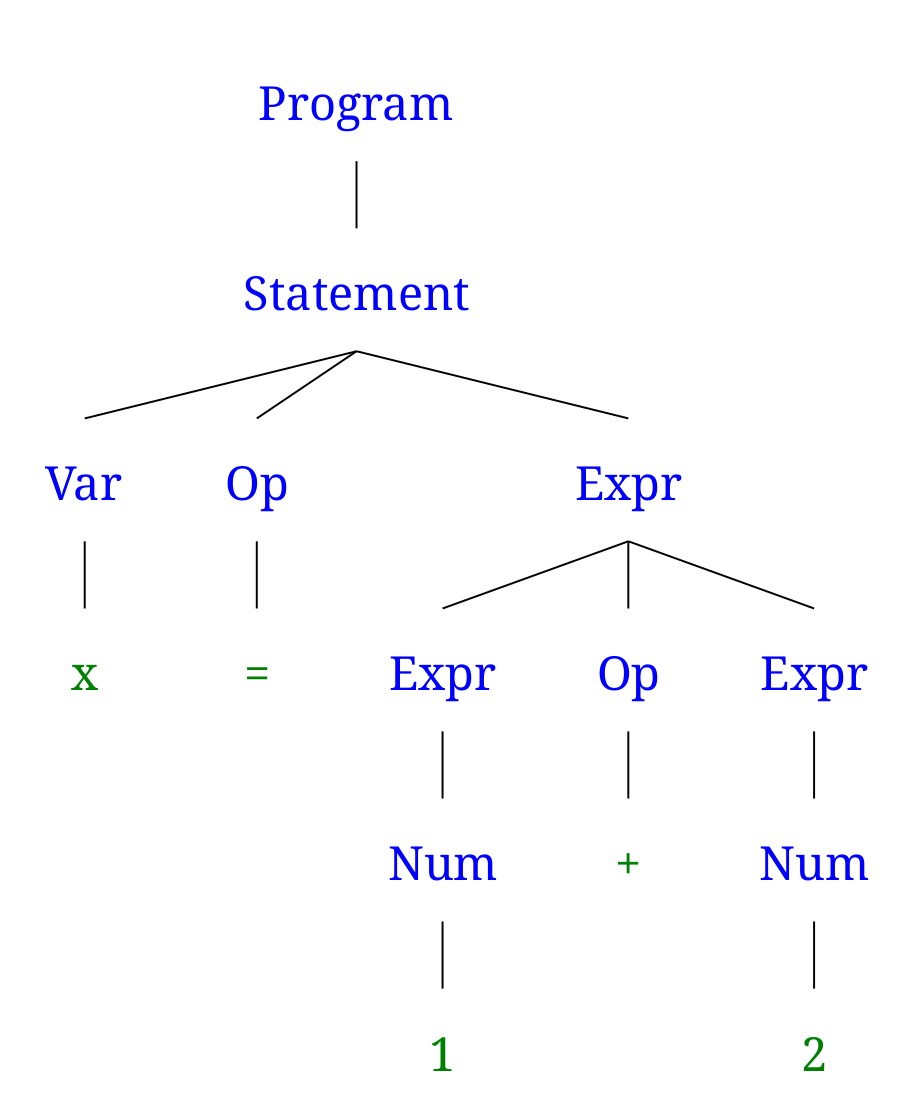
\includegraphics[scale=0.15]{images/parse-tree1.png}
  \caption{Nautilus Seed Representation. This tree represents input seed \texttt{x=1+2}.}\label{nautilus-tree-representation}
\end{figure}
\begin{figure}[h]
  \centering
  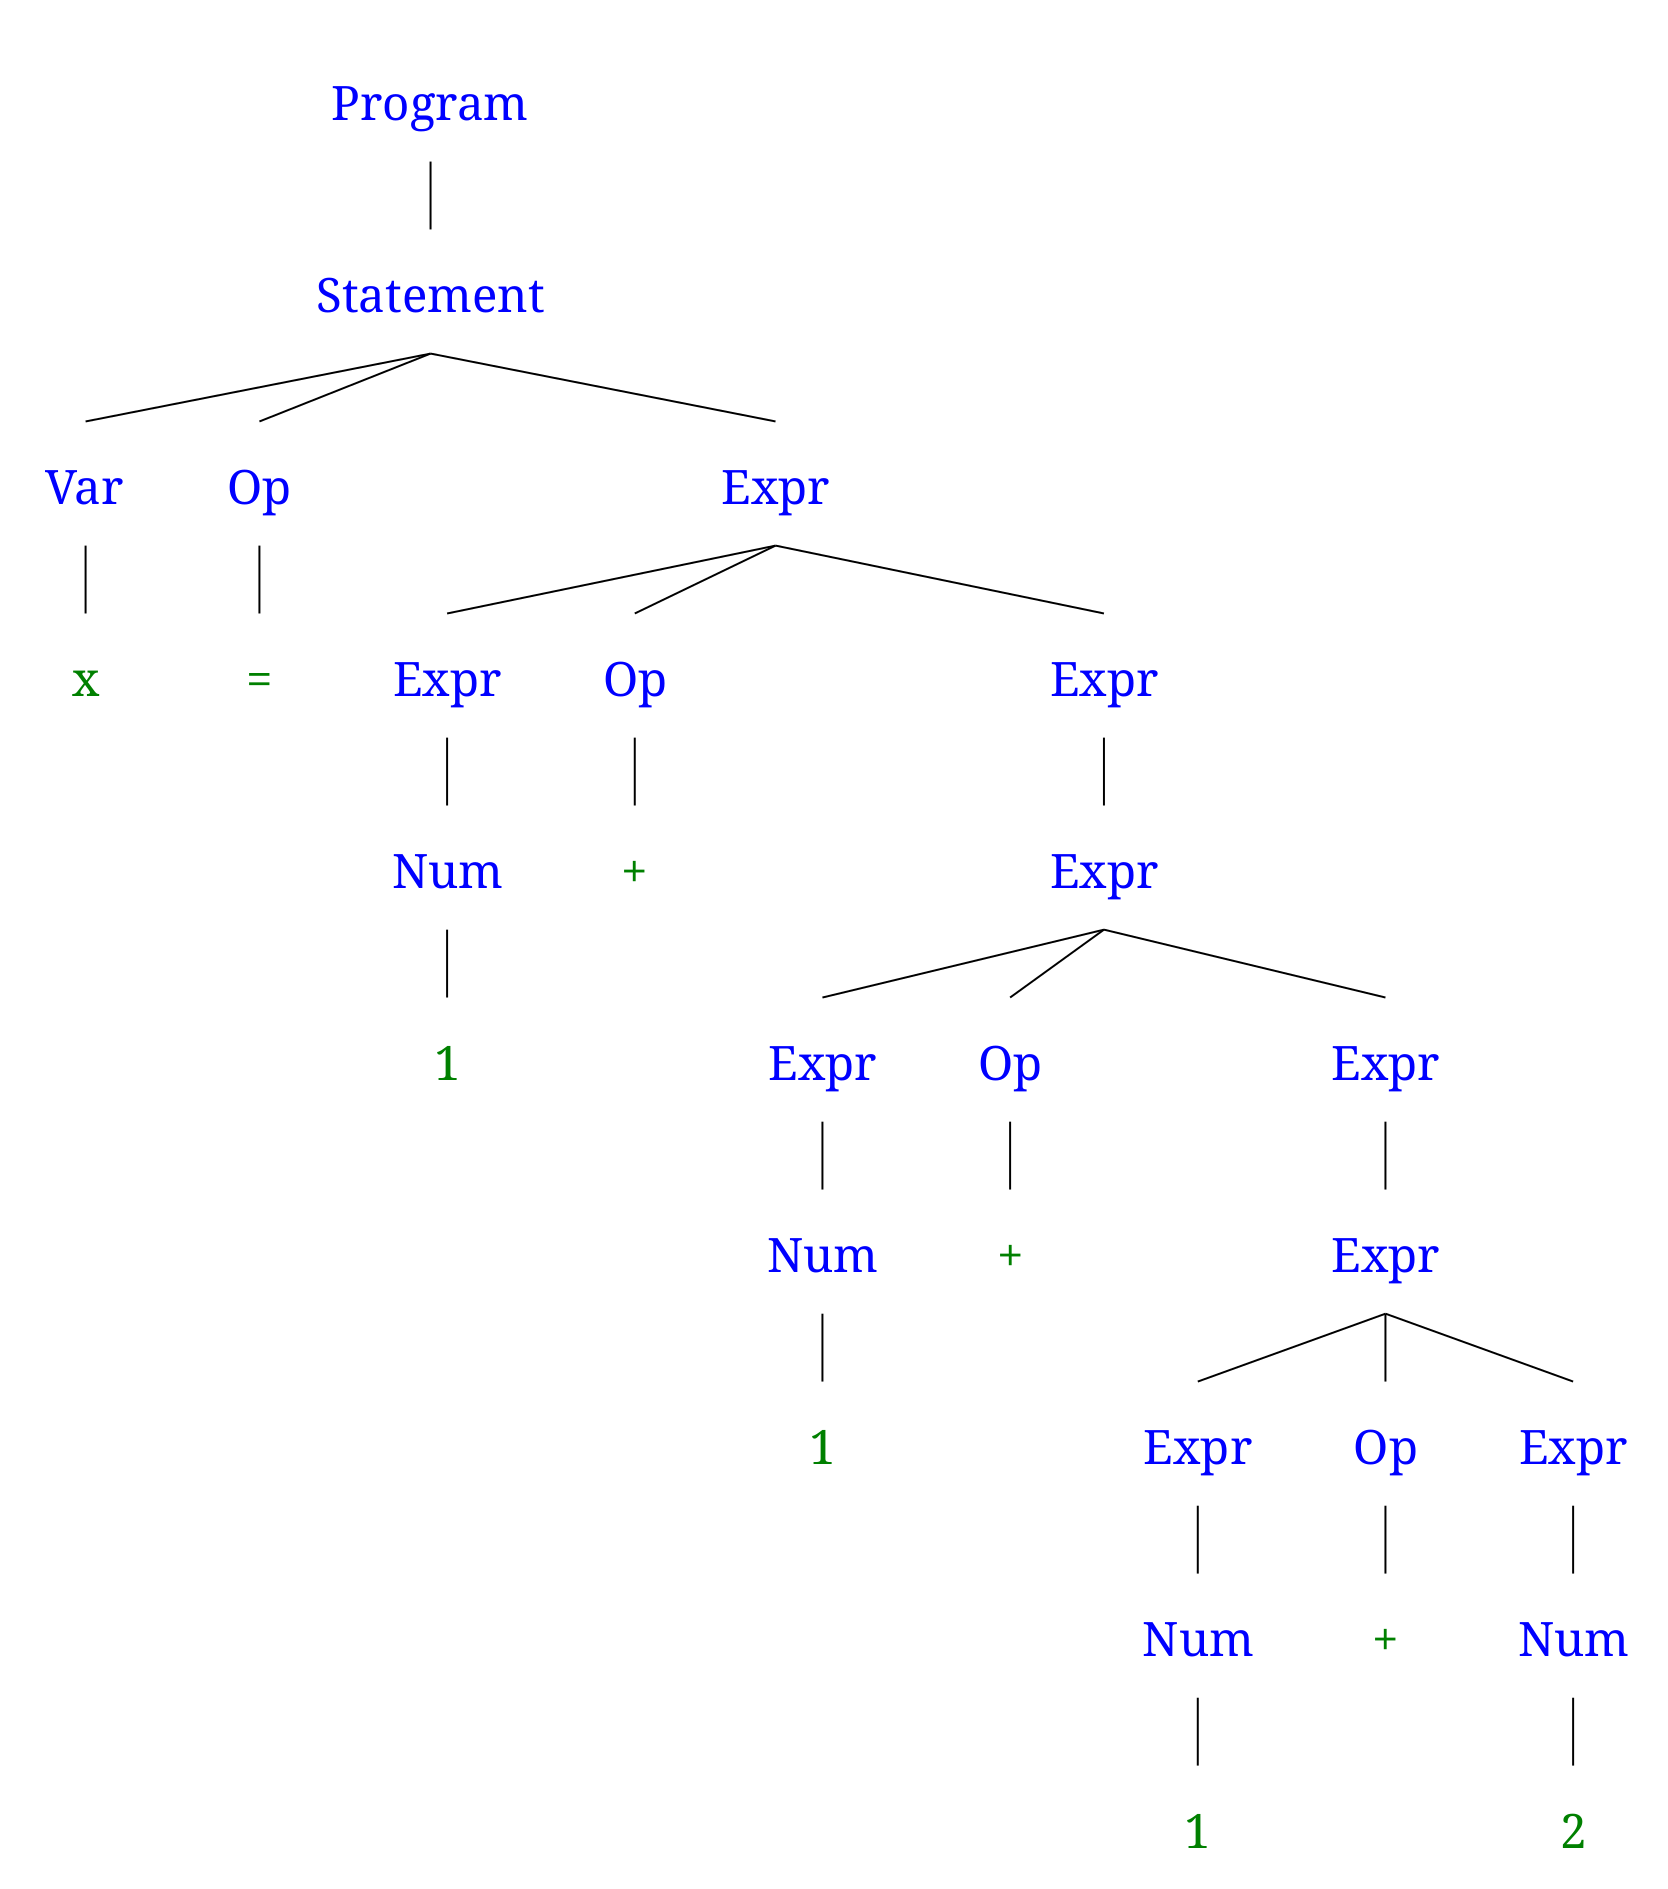
\includegraphics[scale=0.15]{images/parse-tree2.png}
  \caption{Nautilus Random Recursive Mutation. This tree represents the result of recursive mutation from \texttt{x=1+2} to \texttt{x=1+(1+(1+2))}.}\label{nautilus-tree-representation-after-recursive-mutation}
\end{figure}
One important characteristic of Nautilus is that its mutation are often localized. The overhead of making complex changes is big since it requires traversing down the tree to find the right node to mutate. It is also expensive to generate a new tree. Therefore, most of Nautilus' mutations only modify a subtree of the original seed. 

Nautilus has built-in function that can convert an input into tree representation. Therefore, Nautilus can accept user defined seeds.

\paragraph{Gramatron.}
Gramatron is a grammar aware fuzzer that represents the seed inputs as automaton walks \cite{srivastava_payer_2021}. Internally, it converts the input grammar into a finite state automaton (FSA). \figref{example-fsa} shows a subset of PHP grammar as a FSA. For example, \texttt{<?php rand(); ?>} can be represented by automaton walk $[0-1, 1-1, 2-1, 3-1]$.
\begin{figure}[h]
  \centering
  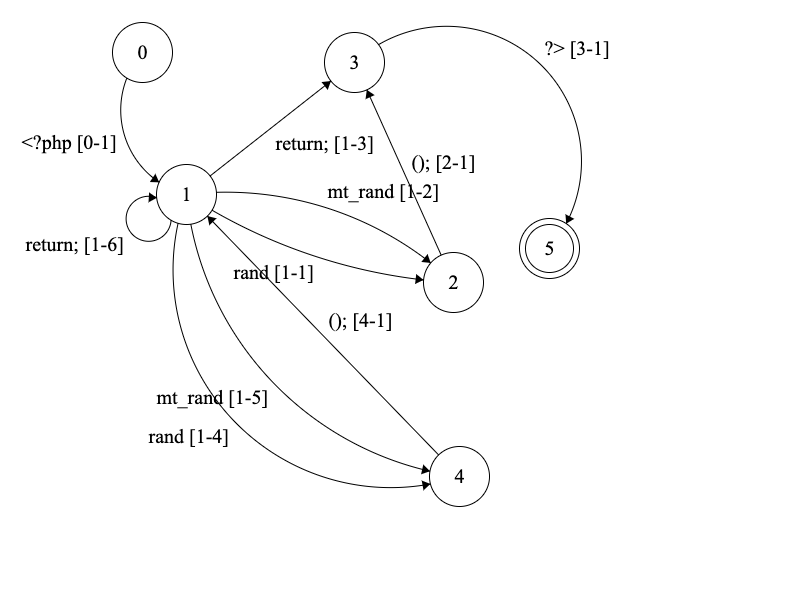
\includegraphics[scale=0.35]{images/fsa.png}
  \caption{Finite State Automaton. This FSA represents a subset of PHP grammar. The indices in the square brackets represent the edges (state transitions) in the graph.}\label{example-fsa}
\end{figure}

Gramatron can perform three kinds of automaton-based mutation.
\begin{enumerate}
    \item Splice. Gramatron replaces part of a seed input's automaton walk with a subwalk from another seed.
    \item Random Mutation. Gramatron chooses a mutation point from the seed's automaton walk, discards the subwalk from that point and starts taking a random walk on the FSA to generate a new subwalk for the seed.
    \item Random Recursion. Gramatron replicates parts of the automaton walk that have recursive features up to $n$ times.
\end{enumerate}

Given an input seed and a point of mutation, Gramatron mutates until the end of the string. The overhead for performing this kind of mutation is smaller using automata than trees since the input is represented by a simple array using automata. This characteristic makes Gramatron's mutation more aggressive than Nautilus'. 

The current implementation of Gramatron does not include function that can parse an input into an automaton walk. Gramatron generates its own input seeds by walking the FSA randomly at the beginning. In this project, I implemented an automaton parser which enables Gramatron to use seeds generated by other mutators.
% Here is how you cite papers. For example, we read papers in the
% class~\cite{rahul2016pwtypos,dodisetal:2004}.  And here is some random citation~\cite{Bojinov:2010:KLP,schechter:2010:pen,everspaugh2015pythia,bellare2009format,Juels:2014}


% \subsection{Overview of the design}
% \label{sec:overview}

% And then just to showoff some \LaTeX skills, here is a Tikz plot.
% % \section{Diagrammatic view of Multisketch operations}\label{app:mainflow}  

% A user registers with a user id $\u$ and a vector of biometric templates
% $\mvec=\mvecss{\mlen}$. Multisketch uses two databases $\dbid$ and $\dbmsg$\@,
% where $\dbid$ contains user id $\u$ and the corresponding helper data
% $\sketchval$, and $\dbmsg$ contains the random permutation of the templates
% registered so far. Highlighted are the entries corresponding to a user $\u_4$
% with templates $\mvec_4=\mvec_{41}\ldots\mvec_{4\mlen}$.% and helper
%     % data $\sketchval_4$.
\begin{figure}[t]
  \centering
  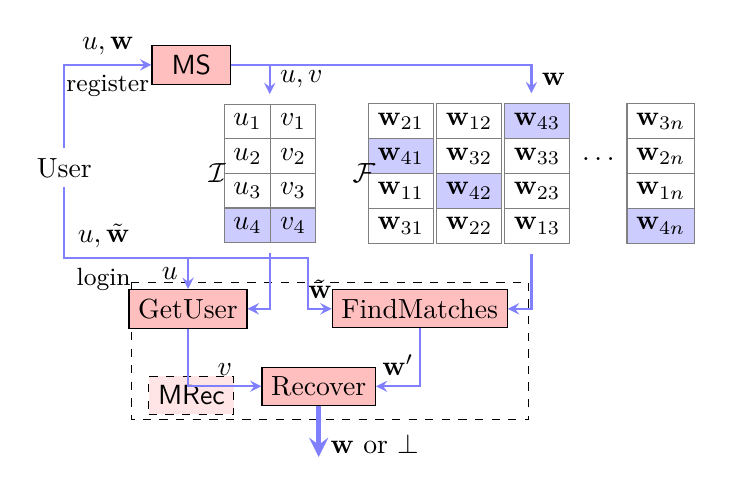
\begin{tikzpicture}[
    >=stealth,
    node distance=2cm,
    database/.style={
      cylinder,
      cylinder uses custom fill,
      cylinder body fill=black!25!white,
      cylinder end fill=black!25!white,
      shape border rotate=90,
      aspect=0.25,
      minimum width=2em,
      minimum height=2em,
      draw
    },
    func/.style={
      rectangle,
      fill=red!25!white,
      minimum width=1cm,
      minimum height=1em,
      draw
    },
    cell/.style={
      rectangle,
      draw=black!50!white
    }
    ]
    \node (user) at (0, 0) {User};
    \node[func, right of=user, right=-1.1em, above=3em] (msketch) {$\MS$}; 
    \draw[below of=msketch, dashed, anchor=west] (.85,0.55) rectangle (5.9,-1.2); 
    \node[func, below of=msketch, anchor=east, below=1.95cm,fill=red!10!white,dashed] (mrecover) {$\MRec$};
    % \node[database, right of=user, anchor=south, above=1em, right=2cm] (db1) {$\dbid$};
    \matrix (db1) [right of=user, anchor=south, below=2pt, right=-0.1cm, 
    matrix of math nodes,
    column sep = -\pgflinewidth,
    row sep=-\pgflinewidth,
    column 1/.style={nodes={cell}}, 
    column 2/.style={nodes={cell}}, 
    anchor=west] {
      \u_1 & \sketchval_1\\
      \u_2 & \sketchval_2\\
      \u_3 & \sketchval_3\\
      |[draw,fill=blue!20]|\u_4 & |[draw,fill=blue!20]|\sketchval_4\\
    };
    \node[left of=db1, anchor=east,right=1.1cm] {$\dbid$};
    \matrix (db2) [right of=db1, left=25pt, matrix of math nodes,
    column sep = 2\pgflinewidth,
    row sep=-\pgflinewidth,
    column 1/.style={nodes={cell}},
    column 2/.style={nodes={cell}}, 
    column 3/.style={nodes={cell}}, 
    column 4/.style={nodes={cell}}, 
    column 5/.style={nodes={cell}}, 
    anchor=west] {
      \mvec_{21} &\mvec_{12} & |[draw,fill=blue!20]|\mvec_{43} &  & \mvec_{3\mlen} \\
      |[draw,fill=blue!20]|\mvec_{41} &\mvec_{32} & \mvec_{33} & |[draw=white]|\ldots & \mvec_{2\mlen} \\
      \mvec_{11} &|[draw,fill=blue!20]|\mvec_{42} & \mvec_{23} &  & \mvec_{1\mlen} \\
      \mvec_{31} &\mvec_{22} & \mvec_{13} & & |[draw,fill=blue!20]|\mvec_{4\mlen} \\
    };
    \node[left of=db2, left=-4pt] {$\dbmsg$};

    % \node[database,right of=db1] (db2) {$\dbmsg$};
    \node[func,below of=db1,anchor=north,above=8pt,left=8pt] (gu) {GetUser};
    \node[func,right of=gu,anchor=east,right=-5pt] (fm) {FindMatches};
    \node[func,below of=db1,anchor=east,below=2em,right=-3pt] (recover) {Recover};

    \draw[->,blue!50,thick] (user.north) |- node[black,near end,above]{$u, \mvec$} node[black,near end,below,font=\small]{register} 
    (msketch.west);
    \draw[->,blue!50,thick] (msketch) -| node[black,near end, left,right]{$u, \sketchval$} (db1);
    \draw[->,blue!50,thick] (msketch) -| node[black,near end, left,right]{$\mvec$} (db2);

    \draw[->,blue!50,thick] (user.south) |- ++(1,-0.9) node[black,near end,above]{$u, \mvectilde$} node[black,near end,below,font=\small]{login}   -| node[black,left,near end]{$u$}
    (gu.north);
    \draw[->,blue!50,thick] (user.south) |- ++(0,-0.9)  -- ++(3.1,0) |- node[black,near end, above]{$\mvectilde$}
    (fm.west);
    \draw[->,blue!50,thick] (db1.south) |- node[black,near end,above]{} (gu.east);
    \draw[->,blue!50,thick] (db2.south) |- node[black,near end,above]{} (fm.east);
    \draw[->,blue!50,thick] (gu.south) |- node[black,near end,above]{$\sketchval$} (recover.west);
    \draw[->,blue!50,thick] (fm.south) |- node[black,near end,above]{$\mvec'$} (recover.east);    
    \draw[->,blue!50,line width=2pt] (recover.south) -- node[black,near end,right]{$\mvec$ or $\bot$} ++(0, -0.65);
  \end{tikzpicture}
  % \rcnote{Rough sketch of the flow of the \biosketch.} 
  \caption{Diagram of multisketch as a part of an authentication service. 
  }
  \label{fig:mainflow}
\end{figure}

%%% Local Variables:
%%% mode: latex
%%% TeX-master: "../main"
%%% End:


% You refer to a figure in the following way. In~\figref{fig:mainflow} we show
% some thing that is relevant for the Multisketch paper by Chatterjee et
% al.~\cite{chatterjee2019multisketches}. Add your bibliography to the
% \textsf{bib.bib} file. You can copy the Bibtex format citation from Google
% Scholar.

%%%%%%%%%%%%%%%%%%%%%%%%%%%%%%%%%%%%%%%%%%%%%%%%%%%%%%%%%%%%%%%%%%%%%%%%%%%%%%%%
\section{Methodology}
\label{sec:methodology}
I propose two approaches to combine Gramatron and Nautilus. First, I wrote a script that pipelines their execution without modifying any internal implementation. This method is easy to implement, but it incurs overhead caused by starting AFLplusplus twice during fuzzing. This method also has the limitation of only being able to run Gramatron before Nautilus because Gramatron cannot take seeds from other mutators. The second method allows Gramatron and Nautilus to run alternately. I modified Gramatron's internal implementation by adding an automaton parser. Without any addition to Gramatron's source code, Gramatron and Nautilus cannot run together because Gramatron cannot parse seeds generated by Nautilus into automaton representations. Once Gramatron is able to obtain these representations, it can mutate seeds generated by other sources and thus run together with Nautilus in one AFLplusplus fuzzing campaign. 

\subsection{Tool Pipeline}
The pipeline approach to combining Gramatron and Nautilus is shown in \figref{tool-pipelining}.
\begin{figure}[h]
  \centering
  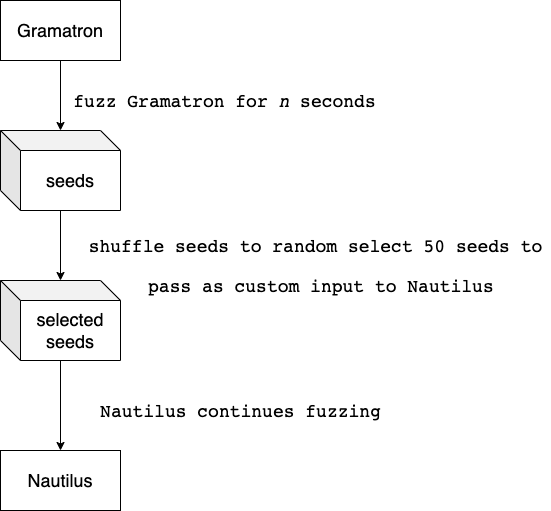
\includegraphics[scale=0.4]{images/pipeline.png}
  \caption{Tool Pipelining.}\label{tool-pipelining}
\end{figure}
The first step is to run Gramatron for a fixed amount of time that is determined heuristically. Then, shuffle the seeds generated by Gramatron to randomly select 50 seeds from the queue to feed into Nautilus. Nautilus can then continue fuzzing on top of Gramatron's generated results. 

This approach to combining the two fuzzers is easy to implement, but it suffers from the following problems.
\begin{enumerate}
    \item Additional time overhead is introduced because AFLplusplus is started twice in each fuzzing campaign. 
    \item The time used to fuzz Gramatron is determined heuristically. It is difficult to decide when is the right time to switch over to Nautilus. If Gramatron is run for too long, the crash might occur before Nautilus is even run, and we lose the benefit we could gain from Nautilus' localized search. On the other hand, if Gramatron is run for only a short time, most of the fuzz work would fall on Nautilus and we lose the benefit from Gramatron's aggressive mutator.
    \item The sequence of running Gramatron and Nautilus is fixed. 
\end{enumerate}

\subsection{Automaton Parser}
To enable Gramatron to accept seeds generated by other mutators, I implemented an automaton parser inside Gramatron. Internally, Gramatron keeps a data structure that stores the FSA representation of the input grammar. The process of learning the automaton walk is essentially a depth first search. The automaton learner parser in the following steps.
\begin{enumerate}
    \item Start from the starting state of the FSA.
    \item Start from the position in the input seed that hasn't been read so far, greedily match the content of the input seed with the symbols of the input language until the next symbol \texttt{s} in the input seed is found. \label{dfs-2}
    \item Iterate through all the out going edges connected to the current state. Each edge has a symbol associated with it as shown in \figref{example-fsa}. Multiple edges that represent the same symbol can be present, so different edges could be explored before the right one is found. If the current symbol \texttt{s} matches the an edge, advance to the state the edge links to and move the position in the input seed, record the edge taken and go to step \ref{dfs-2}. If no edge matches \texttt{s}, discard the current path. 
    \item If the end of the input seed is reached, check if the current state is the accepting state. If the path is accepted, return the current automaton walk. If not, discard the current path.
\end{enumerate}
After an input seed is parsed into an automaton walk, Gramatron would store the walk into a binary file for future reference.

\subsection{Integration inside AFLplusplus}
AFLplusplus has implemented the API that allows users to use one or more custom mutators. \figref{aflplusplus} shows how AFLplusplus works with both Gramatron and Nautilus.

\begin{figure}[]
  \centering
  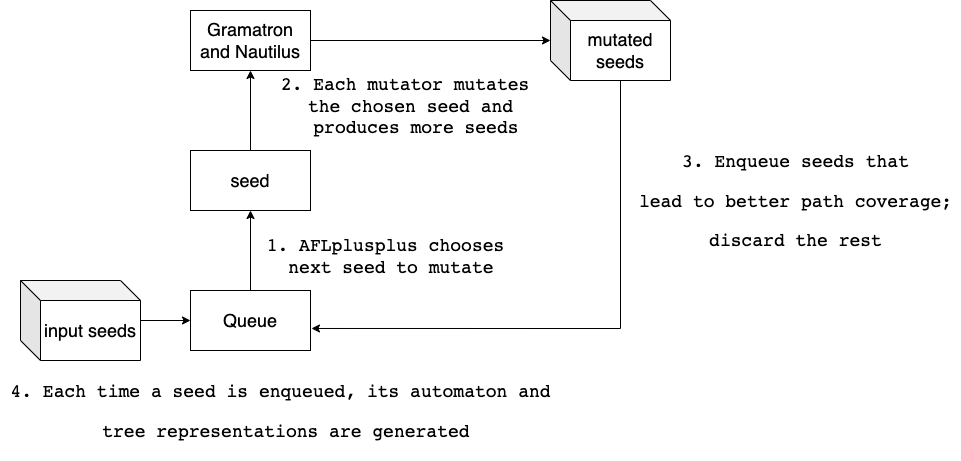
\includegraphics[scale=0.28]{images/AFLplusplus.png}
  
  \caption{AFLplusplus with both Gramatron and Nautilus.}\label{aflplusplus}
\end{figure}

The user would first provide a set of input seeds that comply with the input grammar. All the initial seeds are euqueued into AFLplusplus' internal queue. Every time a seed is enqueued, its automaton and tree representations are generated. During a fuzzing campaign, AFLplusplus first picks a seed from the queue to fuzz. Both Gramatron and Nautilus would be run on each seed to produce more seeds. AFLplusplus then inspects each new seed and enqueue the ones that lead to better path coverage. Since now Gramatron and Nautilus can read each other's seeds, this second method allows Gramatron and Nautilus to run alternately.



%%%%%%%%%%%%%%%%%%%%%%%%%%%%%%%%%%%%%%%%%%%%%%%%%%%%%%%%%%%%%%%%%%%%%%%%%%%%%%%%
\section{Evaluation}
\label{sec:eval}
My evaluation answers whether running the aggressive mutation by Gramatron and the localized search by Nautilus together can generate crashing inputs faster. I used seven different fuzz targets for this evaluation, JS-1, JS-3, JS-4, mruby-1, mruby-2,  PHP-1 and PHP-2 as in \cite{srivastava_payer_2021}. The numbers indicate the different buggy versions of the language interpreter. Some versions have more complex bugs while others have simpler bugs. The complexity of the bugs shown in the third column of Table \ref{fuzz-targets} are gauged by the minimum number of branching rules in the language's CFG to generate a proof of concept crashing input. Table \ref{fuzz-targets} contains more information about the fuzz targets.
\begin{table}[h]
\caption{Fuzz Targets}
\centering
\begin{tabular}{lll}
\hline
Fuzz Target ID & Bug Type             & \begin{tabular}[c]{@{}l@{}}Complexity\\ (Branching Rules)\end{tabular} \\ \hline
PHP-1          & Segmentation Fault   & 15 (Simple)                                                                                                          \\
PHP-2          & Division by Zero     & 15 (Simple)                                                                                                          \\
mruby-1        & Use-after-free       & 27 (Complex)                                                                                                         \\
mruby-2        & Segmentation Fault   & 8 (Simple)                                                                                                           \\
JS-1           & Heap buffer overflow & 26 (Complex)                                                                                                         \\
JS-3           & Failed assertion     & 12 (Simple)                                                                                                        \\ 
JS-4 & Floating point error & 12 (Simple)
                                \\
\hline

\end{tabular}\label{fuzz-targets}
\end{table}
The efficiency of the different mutator tools are evaluated by the time it takes to generate the first crashing input.

\subsection{Benchmark Performance}
To compare if the combination of Gramatron and Nautilus results in an improvement in performance, we need to first have a benchmark performance to compare with. I have run Gramatron and Nautilus on the seven fuzz targets. Each target is fuzzed five times for a fixed amount of time budget. The time budget is 7200 seconds for complex bugs and 1800 seconds for simple bugs. A fuzzing campaign is considered successful if it generates a crashing input within the time budget. 

% Please add the following required packages to your document preamble:
% \usepackage{multirow}
% \usepackage[normalem]{ulem}
% \useunder{\uline}{\ul}{}
\begin{table*}[]
\centering
\caption{Benchmark Performance}
\begin{tabular}{llllllll}
\hline
\multirow{2}{*}{Fuzz Target ID} & \multirow{2}{*}{Time Budget (s)} & \multicolumn{2}{l}{Successful Campaigns} & \multicolumn{2}{l}{Median Time (s)} & \multicolumn{2}{l}{Average Time (s)} \\
                                &                                  & Gramatron           & Nautilus           & Gramatron         & Nautilus        & Gramatron         & Nautilus         \\ \hline
PHP-1                           & 1800                             & 5/5                 & 2/5                & 384               & 1192            & 340               & 1192             \\
PHP-2                           & 1800                             & 5/5                 & 5/5                & 61                & 73              & 67                & 136              \\
mruby-1                         & 7200                             & 4/5                 & 3/5                & 4596              & 2769            & 4121              & 2773             \\
mruby-2                         & 1800                             & 5/5                 & 2/5                & 223               & 762             & 317               & 762              \\
JS-1                            & 7200                             & 5/5                 & 5/5                & 1747              & 729             & 2400              & 784              \\
JS-3                            & 1800                             & 5/5                 & 5/5                & 44                & 34              & 82                & 29               \\
JS-4                            & 1800                             & 5/5                 & 5/5                & 13                & 273             & 35                & 233              \\ \hline
\end{tabular}
\label{tab:benchmark}
\end{table*}
Table \ref{tab:benchmark} shows the benchmark result run on both tools. The benchmark result shows that neither tool outperforms the other in all seven fuzz targets. Gramatron is better in terms of reliability since it only has one failed fuzzing campaign whereas Nautilus has 8 in total. Gramatron is able to produce a crashing input faster than Nautilus when fuzzing PHP-1, PHP-2, mruby-2, and JS-4 while Nautilus performs better when fuzzing mruby-1, JS-1 and JS-3. This result suggests that one fuzzer doesn't always outperform the other and shows promise that combining the two might lead to a faster generation of crashing inputs.

\subsection{Tool Pipeline Performance}
The performance of pipelining both Gramatron and Nautilus is shown Table \ref{tab:pipeline}. For each fuzz target, the runtime for Gramatron is fixed as shown in column 2 in the table. This runtime is determined heuristically by observing data from Table \ref{tab:benchmark}. It should be short enough so that there is a chance that the pipeline method can produce a crashing input sooner than running either fuzzer alone. It should also be long enough because otherwise most of the fuzzing work would fall on Nautilus. After running Gramatron, Nautilus is then given the same time budgets as listed in Table \ref{tab:benchmark}. Sometimes the crashing input would be found by Gramatron before Nautilus is run. The number of this occurrence is written in column 4 of Table \ref{tab:pipeline}. The total runtime is the time from the start of the fuzzing campaign to the time when the first crashing input is produced, which can happen either before or after Nautilus starts to run. 
% Please add the following required packages to your document preamble:
% \usepackage[normalem]{ulem}
% \useunder{\uline}{\ul}{}
\begin{table*}[h]
\caption{Tool Pipelining Performance}
\centering
\begin{tabular}{llllll}
\hline
Fuzz Target ID & Gramatron Runtime (s) & Successful Campaign & Crash in Gramatron & Median Time to Crash in Nautilus & Total Median Time \\ \hline
PHP-1          & 300                   & 2/5                 & 1/5                & 875                              & 826               \\
PHP-2          & 30                    & 5/5                 & 1/5                & 274                              & 304               \\
mruby-1        & 1500                  & 5/5                 & 1/5                & 1941                             & 3188              \\
mruby-2        & 200                   & 4/5                 & 1/5                & 875                              & 1020              \\
JS-1           & 600                   & 5/5                 & 0/5                & 1260                             & 1860              \\
JS-3           & 30                    & 5/5                 & 1/5                & 125                              & 155               \\
JS-4           & 30                    & 5/5                 & 2/5                & 56                               & 46                \\ \hline
\end{tabular}
\label{tab:pipeline}
\end{table*}

% PHP-1: pipelined approach runtime sits in between Gramatron and Nautilus, however successful campaign not good (a lot worse than Gramatron and same with Nautilus). Gramatron not run long enough and Nautilus makes it difficult to find a crashing input within the time budget 
% PHP-2: median time a lot worse than either Gramatron or Nautilus
% mruby-1: median fuzz time better than Gramatron but worse than Nautilus, however provides more stability because all fuzzing campaigns are successful
% mruby-2: median fuzz time median time a lot worse than either Gramatron or Nautilus. Nautilus fuzzed a lot longer than Gramatron. but provided improved stability over running Nautilus alone
% JS-1: median time slightly worse than Gramatron but better in Nautilus
% JS-3: median time much worse than either mutator
% JS-4: median time improved because of running Gramatron.
The pipeline approach performs worse than both Gramatron and Nautilus when fuzzing PHP-2, JS-1 and JS-3. PHP-2 and JS-3 are fuzz targets with simple bugs that only take both fuzzers a few seconds or minutes to generate a crashing target, therefore it is possible that the overhead of pipelining makes the fuzz time longer. In JS-1, the pipeline approach is not outperformed by Gramatron by much, and Nautilus performs a lot worse with the seeds produced by Gramatron than with randomly generated seeds. From Table \ref{tab:benchmark}, we can see that it takes Gramatron almost 2.4 times as long to produce a crashing input than Nautilus. % TODO: the paper provides an explanation
According to \cite{srivastava_payer_2021}, all of the branching rules essential to producing a crashing input for JS-1 are localized within a specific area of the grammar, therefore Gramatron's outputs make it more difficult to produce the crashing input for Nautilus. This makes running Nautilus alone the best way to fuzz JS-1.

The pipeline approach outperforms Nautilus when fuzzing JS-4. Table \ref{tab:benchmark} shows that the median time it takes Nautilus to produce a crashing input is more than 20 times as long as Gramatron, which suggests that Gramatron is better suited to fuzz JS-4. The seeds produced by Gramatron helps Nautilus find bugs easier than with random seeds. The improvement from running the pipeline of the two tools comes mostly from running Gramatron. The pipelined approach outperforms Nautilus in terms of median time when fuzzing PHP-1, but it's just as unstable and is outperformed by Gramatron by a large margin. Table \ref{tab:benchmark} shows that Gramatron is much better at fuzzing PHP-1 than Nautilus, however the effect of running Gramatron is limited in the pipeline approach. This could be because the fixed runtime designated to Gramatron is too short. When fuzzing mruby-2, the median time to find a crashing input with pipeline approach is longer than Gramatron and Nautilus, but it provides more stability compared to Nautilus.

The pipeline approach outperforms Gramatron and is only slightly worse than Nautilus when fuzzing mruby-1. Table \ref{tab:benchmark} shows that Nautilus is better at fuzzing mruby-1 than Gramatron. However, Table \ref{tab:pipeline} shows that Nautilus benefits from seeds generated Gramatron. Although Nautilus is better than the pipeline approach in terms of median time to reach fuzzing input, the pipeline provides more stability than Gramatron and Nautilus when fuzzing mruby-1 since it has succeeded in all fuzzing campaigns.

In general, the pipeline approach sometimes lead to longer median time to both fuzzers, but in some cases it can also outperform one of the two fuzzers and offer better successful campaign rate. It is worth noting that the pipeline approach's performance relies on the runtime allotted to Gramatron. Under different configurations the performance results might change. 
\subsection{Gramatron and Nautilus Integration inside AFLplusplus Performance}
% Please add the following required packages to your document preamble:
% \usepackage[normalem]{ulem}
% \useunder{\uline}{\ul}{}
The performance of using Gramatron and Nautilus as two custom mutators inside AFLplusplus is shown in Table \ref{tab:two-mutator-AFL} \footnote{This part of the evaluation is only done on four fuzz targets because of time constraint of this project}. 
\begin{table*}[]
\caption{Performance of combining two custom mutators inside AFLplusplus}
\begin{tabular}{lllll}
\hline
Fuzz Target ID & Time Budget (s) & Successful Campaigns & Median Time (s) & Average Time (s) \\ \hline
mruby-1        & 7200            & 4/5                  & 4758            & 4375             \\
mruby-2        & 1800            & 3/5                  & 1724            & 1213             \\
JS-1           & 7200            & 5/5                  & 1535            & 1322             \\
JS-4           & 1800            & 5/5                  & 81              & 146              \\ \hline
\end{tabular}\label{tab:two-mutator-AFL}
\end{table*}

For mruby-1, running both Gramatron and Nautilus alternately in one AFLplusplus session leads to a slower discovery of a crashing input compared to the pipeline approach. It is also worse in terms of median time to crash than both Gramatron and Nautilus, but is slightly more stable than Nautilus in terms of successful campaign rate. For mruby-2, running the alternate approach produces the slowest result. It takes the longest time to crash, and although it has a higher successful campaign rate than Nautilus, it is still less stable than Gramatron. For JS-1, the alternate approach outperforms Gramatron and the pipeline approach but legs behind Nautilus. For JS-4, the alternate approach outperforms Nautilus but not Gramatron or the pipeline approach.

Overall, the alternate approach is often outperformed by the pipeline approach, and although it can sometimes lead to faster crash input discovery than one of the tools, it's always worse than the other at the same time. This unsatisfying result might be caused by the following issues.
\begin{enumerate}
    \item The overhead of parsing inputs into automaton walks is big.
    \item A smaller pool of initial seeds is used to keep the size of the queue reasonable.
    \item The pipeline approach allows Gramatron to generate a crashing input before Nautilus is run. Therefore the pipeline approach can make the best use of Gramatron when it can produce a better performance than Nautilus. The alternate approach doesn't have this advantage because the two fuzzers are run in turn.
\end{enumerate}



\section{Conclusion}
\label{sec:conclusion}
This project attempts to combine two popular grammar aware fuzzers, Gramatron and Nautilus, to find bugs faster. From the benchmark performance, it can be observed that Gramatron and Nautilus each have their advantages when fuzzing different targets. When the two tools are run in a pipelined fashion, it results in a better performance than running either Gramatron and Nautilus alone on PHP-1, mruby-1, mruby-2 and JS-4. However, it fails to perform better than both fuzzers on any of the targets in the experiment and it is outperformed by both fuzzers when fuzzing PHP-2, JS-1 and JS-3. The performance of the pipeline approach can be affected negatively due to the overhead of starting AFLplusplus and a non-optimal configuration of Gramatron's runtime, but it also benefits from both the localized mutator and aggressive changes provided by the two tools. The performance of integrating Gramatron and Nautilus inside AFLplusplus is on par with the pipeline approach. It offers some advantage when either Gramatron or Nautilus has a significant advantage over the other on some targets but is also sometimes worse than running both fuzzers individually. Overall, the performance of combining Gramatron and Nautilus fails to meet the expectation of producing a more efficient fuzzer. However, it is worth exploring in the future how the automaton parser can be accelerated, and how the two mutators can be scheduled inside AFLplusplus better for faster discovery of bugs. The source code of this project can be found in \url{https://github.com/yihellen/AFLplusplus/tree/add-automaton-parser}.




%%% Local Variables:
%%% mode: latex
%%% TeX-master: "main"
%%% End:





\bibliographystyle{ACM-Reference-Format}
\bibliography{bib}

% % --- Appendix ---%
\appendix
% \section{Overflow form other sections}
% \label{sec:set-diff-dodis}
% Sometime you ware super excited about some details that does not quite fit with
% the rest of the paper goes here. For example, some details about how you
% instrumented the Android Linux kernel should go to appendix, and for really
% curious reader to read. Remember it's appendix, so the reader is not required to
% read, and you should not put critical information in appendix that is crucial
% for understanding the rest of the paper.




%%% Local Variables:
%%% mode: latex
%%% TeX-master: "main"
%%% End:


\end{document}


%%% Local Variables:
%%% mode: latex
%%% TeX-master: t
%%% End:
